\documentclass[11pt,a4paper]{article}
\usepackage[T1]{fontenc}
\usepackage[utf8]{inputenc}
\usepackage[french]{babel}
\usepackage{lmodern}
\usepackage{amsmath,amssymb}
\usepackage[margin=2.5cm]{geometry}
\usepackage{booktabs}
\usepackage{graphicx}
\usepackage{enumitem}
\usepackage{xcolor}
\usepackage{tabularx}
\usepackage{longtable}
\usepackage{hyperref}
\hypersetup{colorlinks=true,linkcolor=blue!50!black}

\newcommand{\NW}{\mathrm{NW}}
\newcommand{\code}[1]{\texttt{#1}}

\title{Note M4 — Un régime d'avalanches de faillites en loi de puissance,\\
porté par la propagation des pertes de crédit\\
\large Programme M4, workspace \code{m4\_credit\_soc\_fable}}
\author{Agent de recherche M4 (Claude Fable 5)}
\date{14 juillet 2026 --- complété le 17 juillet 2026\\
\small (campagne Simulation Lab $T{=}4000$, 5 seeds par $\lambda$ :
figures d'illustration et lois ajustées)}

\begin{document}
\maketitle

\begin{abstract}
M4 cherchait un régime d'avalanches de faillites auto-organisé : des tailles
d'avalanches en loi de puissance robuste, produites par une dynamique
d'accumulation--relaxation endogène, dépassant nettement le maximum de 7
observé au point de départ. Ce régime est obtenu, avec un moteur
\emph{plus simple} que le point de départ. Trois changements le produisent :
(i)~la fusion des deux variables d'état ($L$, $K$) en une seule (le capital
productif $K$) et la suppression complète de la dette d'amorçage $d_0$ du
code --- le plancher de faillite est purement contractuel ; (ii)~une règle de
faillite \emph{minimale} : à la mort d'une entité, ses créances sont perdues,
les prêts qu'elle portait sont annulés et ses actifs résiduels détruits ---
aucune redistribution ; (iii)~un marché de crédit à \emph{un round
d'appariement par entité et par pas}. Sous chocs purement i.i.d.\ (aucune
corrélation imposée), les tailles d'avalanches causales suivent alors une loi
de puissance d'exposant $\alpha \approx 2{,}4$--$2{,}6$ qui \emph{bat la
log-normale au test de vraisemblance corrigé} ($z$ de $+2{,}3$ à $+57$), dont
la coupure croît avec la taille du système sur toute la gamme testée
(maximum observé : 23--29 à population ${\sim}147$, jusqu'à 224 à population
${\sim}4400$, croissance $\propto N^{0{,}6\text{--}0{,}7}$, sans saturation),
et dont la moitié des membres des grands événements sont des victimes de
cascade (racines/taille $\approx 0{,}5$, profondeur jusqu'à 12). Le rapport
de branchement des cascades s'auto-stabilise à $b = 0{,}30$ sur trente fois
la gamme de taille et sur tous les seeds. Les contraintes du programme sont
préservées : corps de $\NW$ en Fisk, revenu en dPlN, renouvellement complet
du haut de la distribution. En chemin, deux lectures antérieures sont
infirmées : l'axe des chocs sectoriels corrélés produit des \emph{grappes de
morts synchronisées} (racines/taille $=1{,}00$, profondeur $\le 2$), pas des
cascades ; et « la topologie du marché ne compte pas au-delà du volume »
(M3) ne tient pas sous le critère avalanches.
\end{abstract}

\paragraph{Note de révision (17 juillet 2026).} Cette version intègre les
figures d'une seconde campagne confirmatoire, exécutée via l'interface
Simulation Lab : trois lots $\lambda \in \{10, 30, 100\}$ de 5 seeds
chacun, $T = 4000$ pas, configuration finale par défaut (identifiants de
lot en annexe~\ref{sec:annexe-lots}). Chaque assertion quantitative de la
note est désormais illustrée par une figure portant les lois ajustées
(paramètres, $r^2$ et tests en légende) ; sur les tailles d'avalanches,
seules des lois de puissance sont ajustées. Trois compléments de fond,
détaillés aux sections~\ref{sec:volume} et~\ref{sec:distributions} : le
\emph{volume} en joules des avalanches suit, au-dessus d'un mode qui est
une échelle \emph{intensive} (indépendante de la taille du système), une
loi de puissance de pente $-2{,}1$ à $-2{,}3$ ; le revenu au-dessus de
10~J est décrit par un corps exponentiel raccordé à une queue de Pareto
raide (modèle à 3 paramètres, meilleur AIC sur les trois lots) ; et
l'âge au décès est log-normal --- la mortalité n'est pas sans mémoire.

\section{Contexte et objectif}

M3 est un modèle multi-agents de société de crédit : des entités naissent,
produisent, empruntent et prêtent par contrats bilatéraux nominaux, et
meurent par faillite en cascade. Le programme M3 (workspace
\code{m3\_credit\_soc}, notes 01--07) avait établi un générateur
démographique robuste et un canal de crédit distributionnellement actif sous
la règle de revenu (protocole X1), mais \emph{aucune} signature de
criticité auto-organisée (SOC) : les avalanches de faillites restaient
sous-poissoniennes, de taille maximale 7 en baseline.

M4 part d'un fork de M3 et cherche explicitement un régime SOC au sens
opérationnel suivant (brief \code{PROMPT\_M4\_SOC.md}) : distribution des
tailles d'avalanches en loi de puissance (régression log-log de $r^2 > 0{,}90$
hors taille 1, ajustement survivant au test de vraisemblance corrigé),
coupure croissant avec la taille du système, mécanisme
d'accumulation--relaxation endogène articulable (pas une amplification de
corrélation imposée), sans effondrement systémique, et en préservant les
familles de distribution de taille et de revenu des entités ainsi qu'un
renouvellement démographique.

\paragraph{Définitions.} Une \emph{avalanche causale} est une composante
faiblement connexe du graphe des \emph{arêtes de perte} entre entités mortes
à la même résolution de faillites (un pas de temps) : quand l'emprunteuse
$i$ meurt, chaque prêteuse $j$ de $i$ perd sa créance $q_{ij}$, ce qui crée
l'arête $(i \to j)$ ; si $j$ meurt dans la même résolution, $i$ et $j$
appartiennent à la même avalanche. Les \emph{racines} d'une avalanche sont
les entités entrées en faillite à la première itération (insolvabilité ou
défaut de service) ; les autres membres sont des victimes de cascade. La
\emph{profondeur} est le nombre d'itérations de la cascade. Le
\emph{rapport de branchement} empirique est
$b = 1 - \sum \text{racines} / \sum \text{tailles}$ : la fraction des morts
qui sont des victimes induites.

\section{Le modèle final (moteur fusionné, \code{src/m4})}

Chaque entité $i$ possède un unique stock réel, le capital productif
$K_i \ge 0$, et des contrats de prêt nominaux perpétuels $(\ell, b, q, r)$ :
la prêteuse $\ell$ a versé le principal $q$ à l'emprunteuse $b$, qui lui doit
$r q$ d'intérêts par pas. La valeur nette est
$\NW_i = K_i + C_i - D_i$ où $C_i$ (créances) et $D_i$ (dettes) sont les
sommes des principaux prêtés et empruntés. \textbf{Il n'y a pas de dette
d'amorçage $d_0$} : une entité sans dette ne peut pas mourir ; le plancher
d'absorption est purement contractuel (régime validé par l'ablation H de M3
puis par le sweep B de M4).

Séquence d'un pas (paramètres par défaut entre parenthèses) :
\begin{enumerate}[nosep]
\item \textbf{Naissances} : $n \sim \text{Poisson}(\lambda)$ entités, dotation
  $K_0$ ($25$), sans dette.
\item \textbf{Choc} : $K_i \gets K_i e^{\eta_i}$,
  $\eta_i \sim \mathcal{N}(-\sigma^2/2, \sigma^2)$ i.i.d.\ ($\sigma = 0{,}25$)
  --- \emph{aucune} composante commune ou sectorielle en baseline.
\item \textbf{Production} : $K_i \gets K_i + \alpha\sqrt{K_i}$ ($\alpha = 1$),
  entièrement retenue.
\item \textbf{Service des intérêts} : chaque emprunteuse paie
  $\sum_j r_j q_j$ depuis $K$ ; insuffisance $\to$ paiement partiel au
  prorata et \emph{défaut de service}.
\item \textbf{Dépréciation} : $K_i \gets (1-\delta) K_i$ ($\delta = 0{,}05$) ;
  les contrats, nominaux, ne se déprécient pas (asymétrie constitutive).
\item \textbf{Marché} : $\lfloor N \rfloor$ rounds (\emph{un par entité
  vivante}) ; par round, échantillon de $k = 3$ entités, prêteuse $=$ $K$
  maximal, emprunteuse $=$ $K$ minimal, taux $r = \sqrt{r_\ell r_b}$ avec
  $r_x = \alpha/(2\sqrt{K_x})$, cible commune $K^*(r) = (\alpha/2r)^2 =
  \sqrt{K_\ell K_b}$ (règle de revenu X1), volume
  $q = \min(K_\ell - K^*, K^* - K_b)$, transfert réel $K_\ell \to K_b$.
\item \textbf{Faillites en cascade} : entrée si défaut de service ou
  $\NW < 0$ ; à la mort de $i$ : créances sur $i$ perdues (arêtes de perte),
  prêts portés par $i$ \emph{annulés} (gain pour ses emprunteuses), actifs
  résiduels $K_i$ \emph{détruits} ; itération jusqu'au point fixe.
\end{enumerate}

Par rapport au fork M3 de départ, ont disparu : $d_0$, la liquidité $L$ et
ses paramètres ($L_0$, part retenue $s$, consommation $c$, tampon
$\beta_L$), les chocs sectoriels en baseline ($\rho_s = 0$), la
redistribution prorata à la faillite (créances transférées, actifs
récupérés), et cinq options de configuration héritées des ablations M3. Le
moteur L/K complet de départ est archivé
(\code{archive/m4\_lk\_pre\_refonte/}) et la suite de tests (61 tests,
invariants comptables, cascade, réduction sans crédit, estimateurs sur
données synthétiques) est verte.

\section{Le mécanisme, et comment il a été trouvé}

\subsection{Ce qui ne marche pas : la corrélation imposée}

Le point de départ suggéré (chocs sectoriels corrélés, variante G2b de M3,
$\rho_s = 0{,}8$) produit bien des « grosses avalanches » (max 62--89 à
$\lambda = 100$) avec $r^2 > 0{,}90$ hors taille~1 --- mais leur structure
interne les disqualifie : \textbf{racines/taille $= 1{,}00$ et profondeur
$\le 2$ partout}. Ce sont des morts \emph{simultanées}, synchronisées par le
choc commun, que le graphe de pertes relie comptablement via des prêteuses
communes ; il n'y a aucune propagation. La cause est structurelle : avec la
sélection assortative et la redistribution prorata de M3, seules les
entités les plus riches prêtent, et l'exposition maximale d'une prêteuse
vaut en médiane $7\,\%$ de sa valeur nette (aucune prêteuse au-dessus de
$49\,\%$, mesuré sur \code{b\_lam30p0\_s0}) : aucun défaut isolé ne peut
tuer personne. La leçon de méthode : le marqueur $r^2$ hors taille~1 est
nécessaire mais pas suffisant --- il faut vérifier racines/taille et
profondeur.

\subsection{Ce qui marche : des pertes sans amortisseur sur un carnet non fragmenté}

Deux règles de faillite héritées de M2/M3 amortissaient structurellement la
contagion : le \emph{transfert} des prêts de la morte à ses créancières
(qui fragmente le carnet en micro-expositions --- jusqu'à 12,4~M de contrats
sur la grille M3) et la \emph{récupération} prorata des actifs résiduels
(qui rembourse une partie de la perte). En remplaçant les deux par la règle
minimale (annulation + destruction), la propagation apparaît immédiatement :
racines/taille passe de $1{,}00$ à $0{,}44$--$0{,}51$, la profondeur de 2 à
8--12. Aucune des deux ne suffit seule : destruction seule $\to$ distribution
en bosse ($r^2 = 0{,}36$) ; annulation seule $\to$ propagation partielle
(profondeur 4--5, $\alpha \approx 4{,}5$). C'est la combinaison qui fait le
régime --- et elle \emph{simplifie} le code.

\subsection{Le paramètre de contrôle : le volume de crédit ; son réglage naturel}

Le rapport de branchement $b$ répond au volume d'appariement du marché
(rounds par entité et par pas), et à rien d'autre de testé ($\sigma$ de
0,20 à 0,35 ne le déplace pas) :
\[
\begin{array}{lcccccc}
\text{rounds/tête} & 1/6 & 1/3 & 1/2 & 1 & 2 & 4\\
b & 0{,}14 & 0{,}20 & 0{,}24 & 0{,}30 & 0{,}34 & 0{,}36\\
x_c \text{ (coupure ajustée, } \lambda{=}30) & 3 & 8\text{--}10 & 28\text{--}33 &
514\text{--}1019 & \text{(dégradé)} & \text{(bosse)}
\end{array}
\]
La coupure $x_c$ (ajustement loi de puissance $\times$ coupure
exponentielle, §\ref{sec:stats}) monte de deux décades et demie quand le
volume passe de $1/6$ à $1$ round/tête ; au-delà ($2n$, $4n$ rounds), la
distribution se dégrade (bosse, $r^2 \to 0{,}64$) : le marché
« sur-apuré » dépasse légèrement le point critique. \textbf{À un round par
tête --- la normalisation naturelle, pas un réglage fin --- le système est
dans la fenêtre critique, et cette fenêtre est large d'un facteur
${\sim}2$.}

\begin{figure}[htbp]
\centering
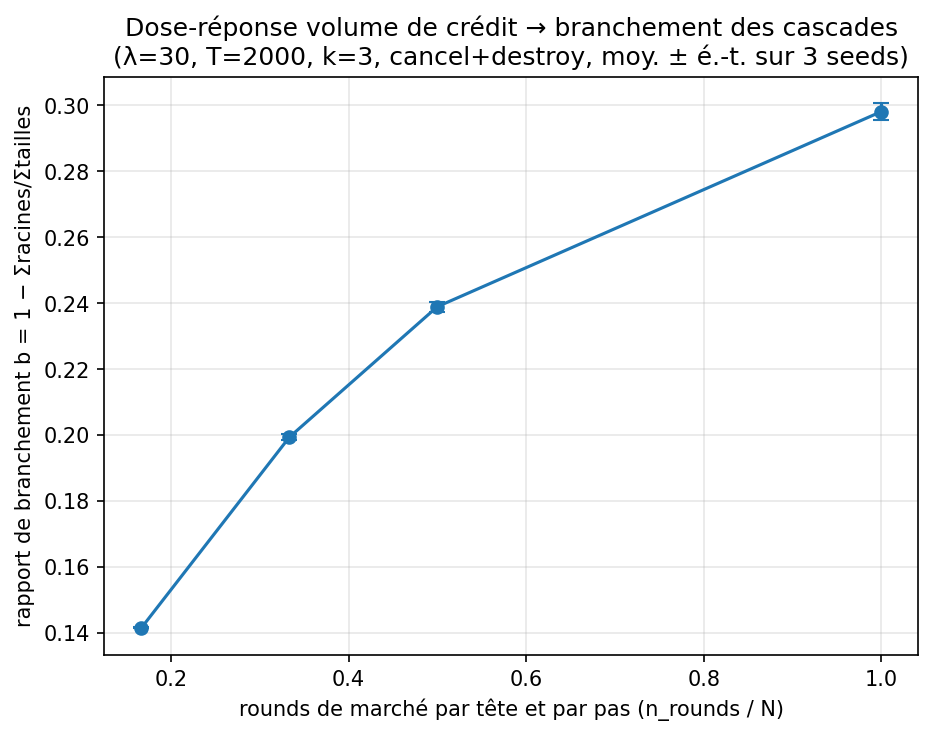
\includegraphics[width=0.72\textwidth]{figures/dose_reponse_volume_b.png}
\caption{Dose-réponse volume de crédit $\to$ rapport de branchement $b$
($\lambda{=}30$, $T{=}2000$, $k{=}3$, annulation$+$destruction ; moyenne
$\pm$ écart-type sur 3 seeds par point ; runs \code{v\_r6/v\_r3/v\_r2} et
\code{f\_lam30}). La coupure $x_c$ associée monte de 3 à ${\sim}10^3$ le
long de cet axe.}
\label{fig:dose}
\end{figure}

\subsection{L'histoire causale, en une phrase}

Pendant les périodes calmes, le marché reconstruit en continu un réseau
dense de créances (accumulation : le carnet croît de $+1$ à $+4$
contrats/pas dans les 20 pas précédant un grand événement, contre une
tendance globale nulle --- mesuré sur ${\sim}390$ événements $\ge 15$ par
seed) ; chaque insolvabilité contractuelle détruit sans amortisseur une
partie du bilan de ses créancières, dont la chute propage la perte le long
des chaînes d'intermédiation (relaxation : profondeur jusqu'à 12, moitié
des membres des grands événements sont des victimes induites) ; la cascade
élague le réseau ($-1$ à $-1{,}4\,\%$ de contrats après l'événement), qui
se reconstruit. Le branchement $b$ s'auto-stabilise à $0{,}300 \pm 0{,}003$
sur trente fois la gamme de taille de système et sur tous les seeds testés
(fig.~\ref{fig:accum} et~\ref{fig:branching}).

\begin{figure}[htbp]
\centering
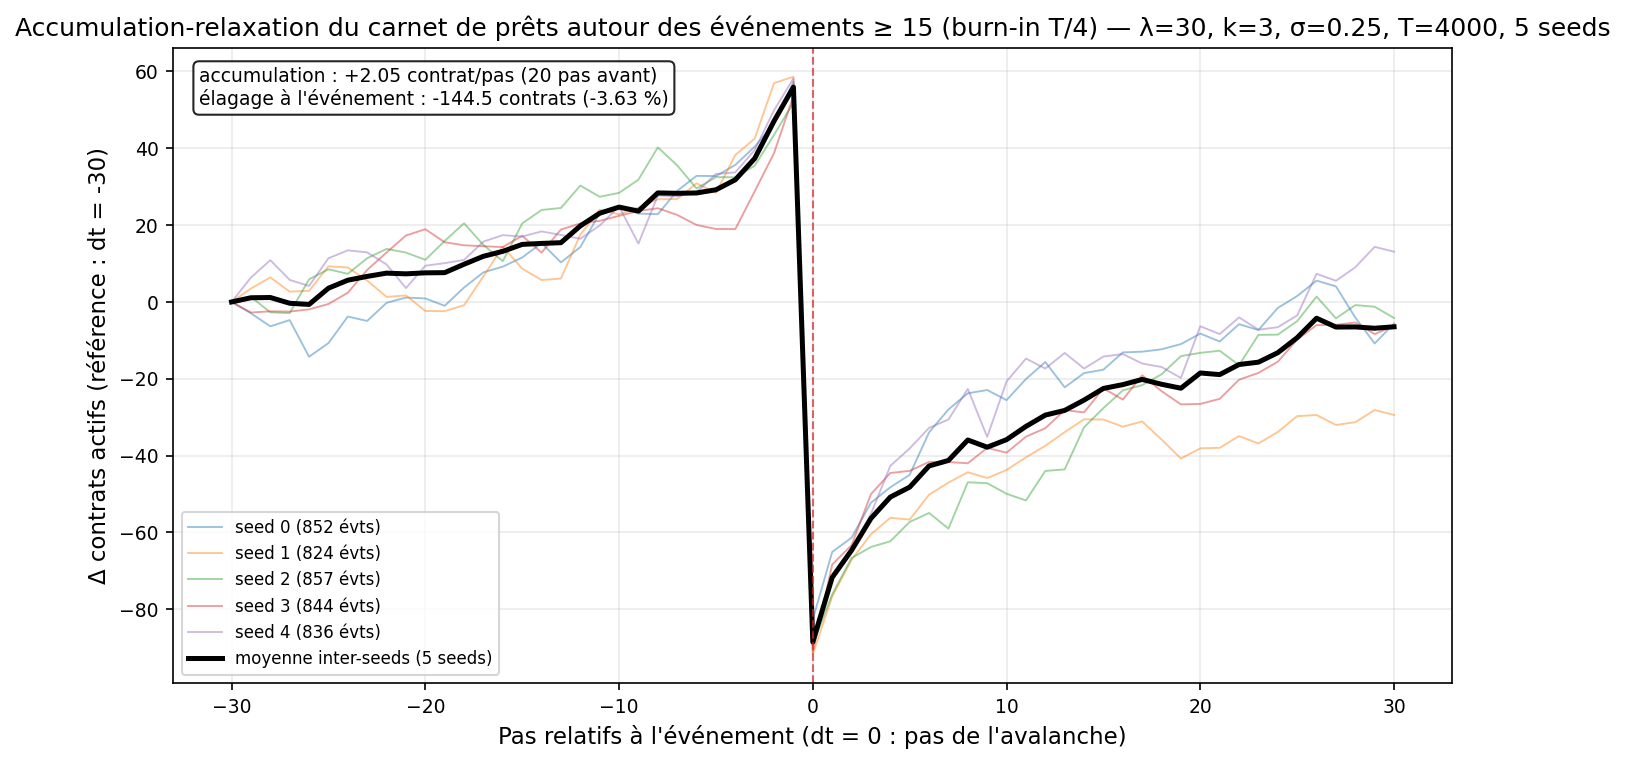
\includegraphics[width=0.95\textwidth]{figures/lot30_accumulation_relaxation.png}
\caption{Cycle accumulation--relaxation, mesuré par analyse d'époques
superposées : nombre de contrats de prêt actifs (carnet), moyenné sur
tous les grands événements ($\ge$ seuil indiqué), aligné sur le pas de
l'événement ($\Delta t = 0$), fenêtre de $\pm 30$ pas, un profil par seed.
Le carnet croît dans les pas qui précèdent un grand événement
(accumulation), chute à l'événement (relaxation par élagage des contrats
des mortes), puis se reconstruit. Lot $\lambda{=}30$, $T{=}4000$, 5 seeds
(lot \code{20260715\_154731}, annexe~\ref{sec:annexe-lots}).}
\label{fig:accum}
\end{figure}

\begin{figure}[htbp]
\centering
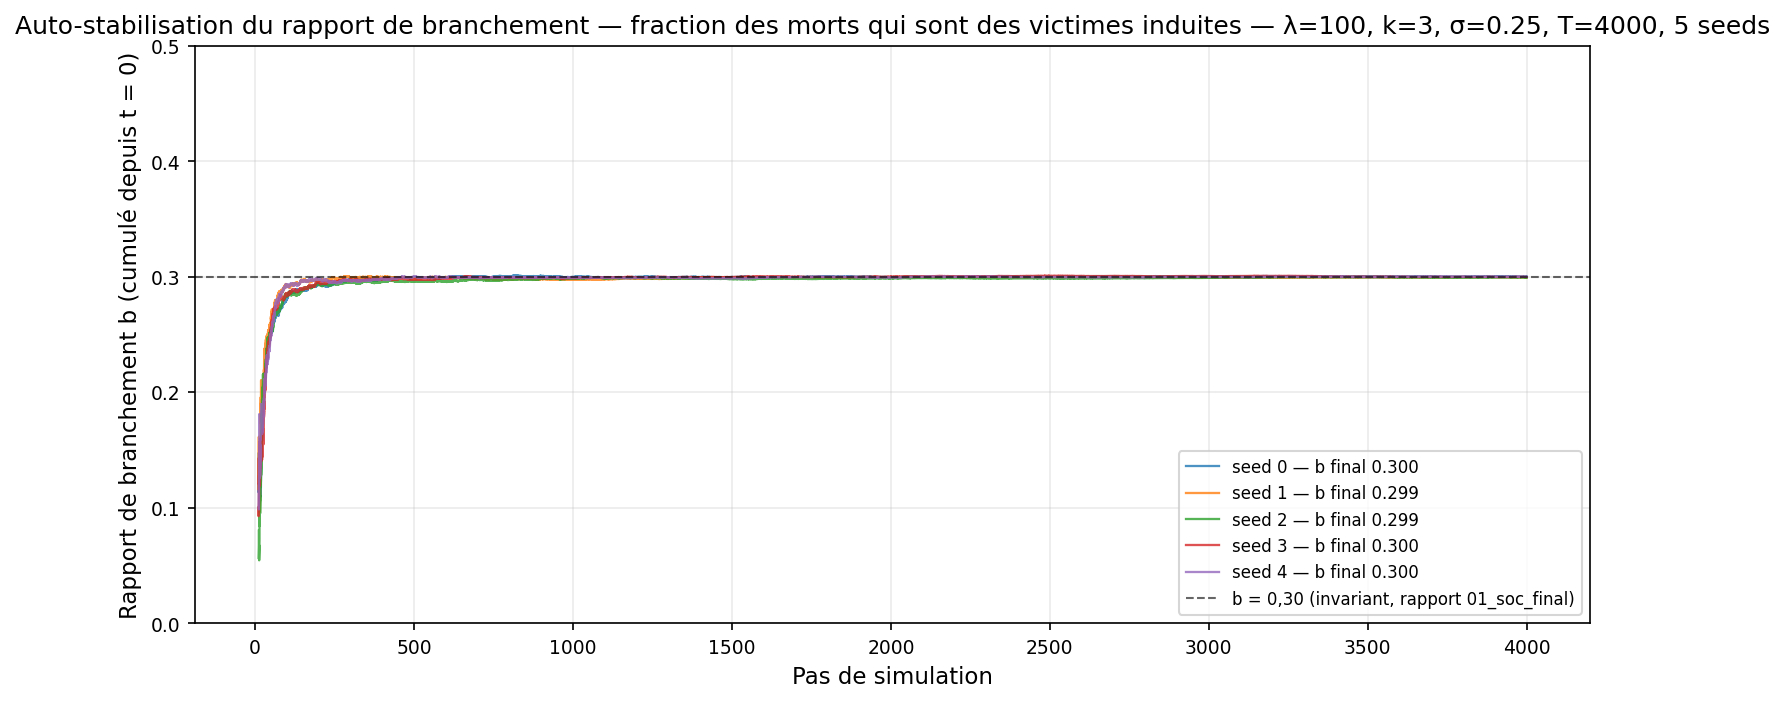
\includegraphics[width=0.8\textwidth]{figures/lot100_branching_ratio.png}
\caption{Auto-stabilisation du rapport de branchement : $b(t)$ cumulé
(fraction des morts qui sont des victimes induites, calculée sur toutes
les avalanches depuis le burn-in jusqu'à $t$) converge vers
${\sim}0{,}30$ pour chacun des 5 seeds, sans qu'aucun paramètre ne soit
ajusté pendant le run. Lot $\lambda{=}100$, $T{=}4000$
(lot \code{20260715\_155159}).}
\label{fig:branching}
\end{figure}

\section{Outillage statistique}
\label{sec:stats}

Les tailles d'avalanches sont des entiers dominés par les singletons : les
estimateurs continus de M2/M3 y dégénèrent (rapport 05 de M3). L'outillage
M4 (\code{experiments/m4/soc\_stats.py}, validé par 8 tests sur données
synthétiques, y compris l'absence de faux positifs) comprend :
\begin{itemize}[nosep]
\item la double régression log-log sur densité log-binnée (avec et hors
  taille 1), reprise des recettes de figures existantes ;
\item le MLE \emph{discret} de la loi de puissance ($p(s) \propto s^{-\alpha}$,
  normalisation par la zêta de Hurwitz, scan du seuil $s_{\min}$ par
  Kolmogorov--Smirnov) ;
\item le test de Vuong loi de puissance vs log-normale \emph{discrète
  renormalisée sur le même support} (le piège n°1 du programme --- la
  log-normale non renormalisée --- est testé explicitement) ;
\item le MLE loi de puissance $\times$ coupure exponentielle
  ($p(s) \propto s^{-\alpha} e^{-s/x_c}$, discret) et son test de Vuong
  contre la log-normale : c'est le verdict honnête en taille finie, la loi
  de puissance \emph{pure} étant mécaniquement battue par la log-normale
  quand $x_c$ est petit devant la gamme.
\end{itemize}
Burn-in : $t \ge T/4$, robustesse vérifiée ($t_{\min} \in \{500, 1000,
1500\}$ : pente $\pm 0{,}3$, $r^2 > 0{,}90$) ; robustesse au temps total
vérifiée ($T = 4000$ : $\alpha$ et structure inchangés).

\section{Résultats de la campagne confirmatoire (config finale)}

Campagne F : $\lambda \in \{10, 30, 100\} \times 3$ seeds $+$ $\lambda = 300$
(seed 0) $+$ $T = 4000 \times 3$ seeds, $T = 2000$ sinon. Tous les artefacts
sur disque (\code{experiments/m4/results/f\_*}).

\paragraph{Seconde campagne confirmatoire (Simulation Lab, 17 juillet).}
Trois lots $\lambda \in \{10, 30, 100\} \times 5$ seeds, $T = 4000$,
configuration finale (annexe~\ref{sec:annexe-lots}) rejouent tous les
critères avec une statistique double : $\alpha$ (MLE discret,
$s_{\min}{=}1$) $= 2{,}38$--$2{,}54$ ; $z$ de Vuong $+3{,}0$
($\lambda{=}10$) à $+49{,}2$ ($\lambda{=}100$) ; $r^2$ hors taille~1
$= 0{,}92$--$0{,}97$ ; $b = 0{,}292$--$0{,}301$ ; racines/taille
$= 0{,}48$--$0{,}51$ ; profondeur maximale 9--14 ; coupure ajustée $x_c
= 33$--$41$ ($\lambda{=}10$), $575$--$961$ ($\lambda{=}30$), au-delà de la
gamme observable ($\lambda{=}100$) ; maximum $\propto N^{0{,}59}$ ;
population stationnaire à ${\sim}14{,}7$ vivantes par unité de $\lambda$.
Les figures~\ref{fig:hist-fits} à~\ref{fig:structure} illustrent ces
chiffres.

\begin{center}
\begin{tabular}{lccccccc}
\toprule
$\lambda$ & pop.\ moy. & max & $\alpha$ (MLE discret) & LR pur $z$ &
$b$ & rac./taille & prof.\ max\\
\midrule
10 & 146--148 & 23--29 & 2{,}39--2{,}42 & $+2{,}3$ à $+4{,}6$ & 0{,}29 & 0{,}48--0{,}49 & 8--9\\
30 & 444--446 & 46--60 & 2{,}43--2{,}45 & $+15{,}6$ à $+18{,}1$ & 0{,}30 & 0{,}49--0{,}50 & 9--12\\
100 & 1472--1477 & 108--111 & 2{,}54 & $+34{,}4$ à $+34{,}5$ & 0{,}30 & 0{,}51 & 11\\
300 & 4414 & 224 & 2{,}63 & $+57{,}2$ & 0{,}30 & 0{,}51 & 12\\
\bottomrule
\end{tabular}
\end{center}

\begin{figure}[htbp]
\centering
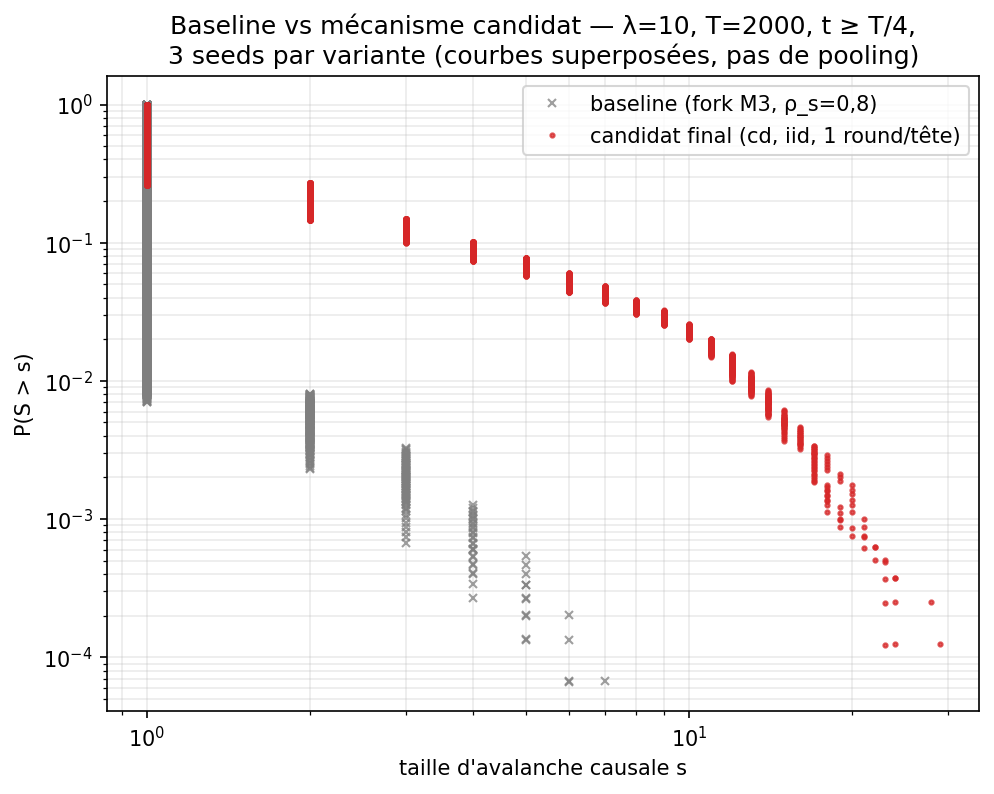
\includegraphics[width=0.65\textwidth]{figures/baseline_vs_candidat_ccdf.png}\\[4pt]
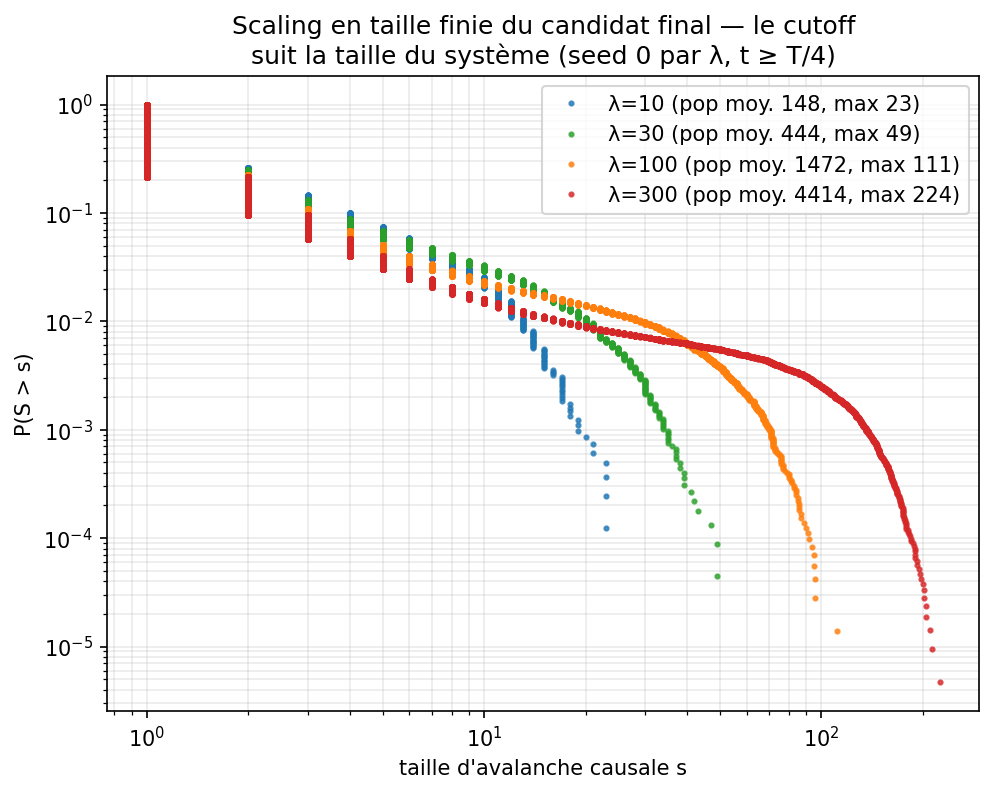
\includegraphics[width=0.65\textwidth]{figures/candidat_scaling_ccdf.png}
\caption{Haut : fonctions de survie $P(S > s)$ des tailles d'avalanches,
baseline du fork (moteur L/K, chocs sectoriels $\rho_s = 0{,}8$, max 7) vs
candidat final (chocs i.i.d., max 23--29), à $\lambda = 10$, 3 seeds par
variante. Bas : scaling en taille finie du candidat final --- corps commun,
décollement à une coupure qui suit la taille du système (max 23 $\to$ 224
pour pop.\ 148 $\to$ 4414).}
\label{fig:ccdf}
\end{figure}

\begin{itemize}[nosep]
\item \textbf{Critère 1} (marqueur principal) : $r^2$ hors taille 1
  $= 0{,}92$--$0{,}98$ sur les 10+ runs ; les régressions avec et sans
  taille 1 coïncident désormais (l'excès de singletons du régime M3 a
  disparu).
\item \textbf{Critère 2} (scaling) : le maximum croît de 23 à 224 sur la
  gamme, $\propto N^{0{,}6\text{--}0{,}7}$, sans saturation ; la coupure
  ajustée $x_c$ passe de ${\sim}35$ ($\lambda{=}10$) à
  ${\sim}500$--$1000$ ($\lambda{=}30$) puis dépasse la gamme observable
  ($\lambda \ge 100$ : ajustement non borné).
\item \textbf{Critère 3} (LR corrigé) : la loi de puissance \emph{pure} bat
  la log-normale discrète renormalisée partout ($z > 2$), de plus en plus
  nettement avec la taille.
\item \textbf{Critère 7} (anti-effondrement) : chute maximale de population
  en un pas : $2$--$9\,\%$ ; population stationnaire ; le plus grand
  événement emporte au plus ${\sim}16\,\%$ de la population ($\lambda=10$),
  $5\,\%$ à $\lambda=300$. Nuance : la CCDF à $\lambda \ge 100$ montre un
  \emph{épaulement} avant la coupure (fig.~\ref{fig:ccdf}, accumulation
  d'événements quasi-systémiques --- attendu en taille finie près de la
  criticité, et cohérent avec le $r^2$ légèrement plus bas, 0,95--0,96) ;
  ce n'est pas la bimodalité « masse de singletons $+$ effondrement total »
  contre laquelle le brief met en garde, mais c'est à surveiller aux tailles
  supérieures.
\item \textbf{Exposant} : au seuil $s_{\min}=1$, $\alpha$ semble dériver
  avec la taille (2,40 $\to$ 2,63) ; c'est un artefact du poids des
  singletons --- à $s_{\min} = 2$, $\alpha = 2{,}26$--$2{,}32$ sur toute la
  gamme (à $s_{\min} = 3$ : 2,18--2,41, dérive inversée) : l'exposant de
  queue est ${\sim}2{,}2$--$2{,}3$, les variations résiduelles étant de
  l'ordre des corrections de coupure.
\item \textbf{Structure causale} : la moitié des membres des événements
  $\ge 5$ sont des victimes de cascade ; profondeur maximale 8--12,
  croissante avec la taille de système.
\end{itemize}

\begin{figure}[htbp]
\centering
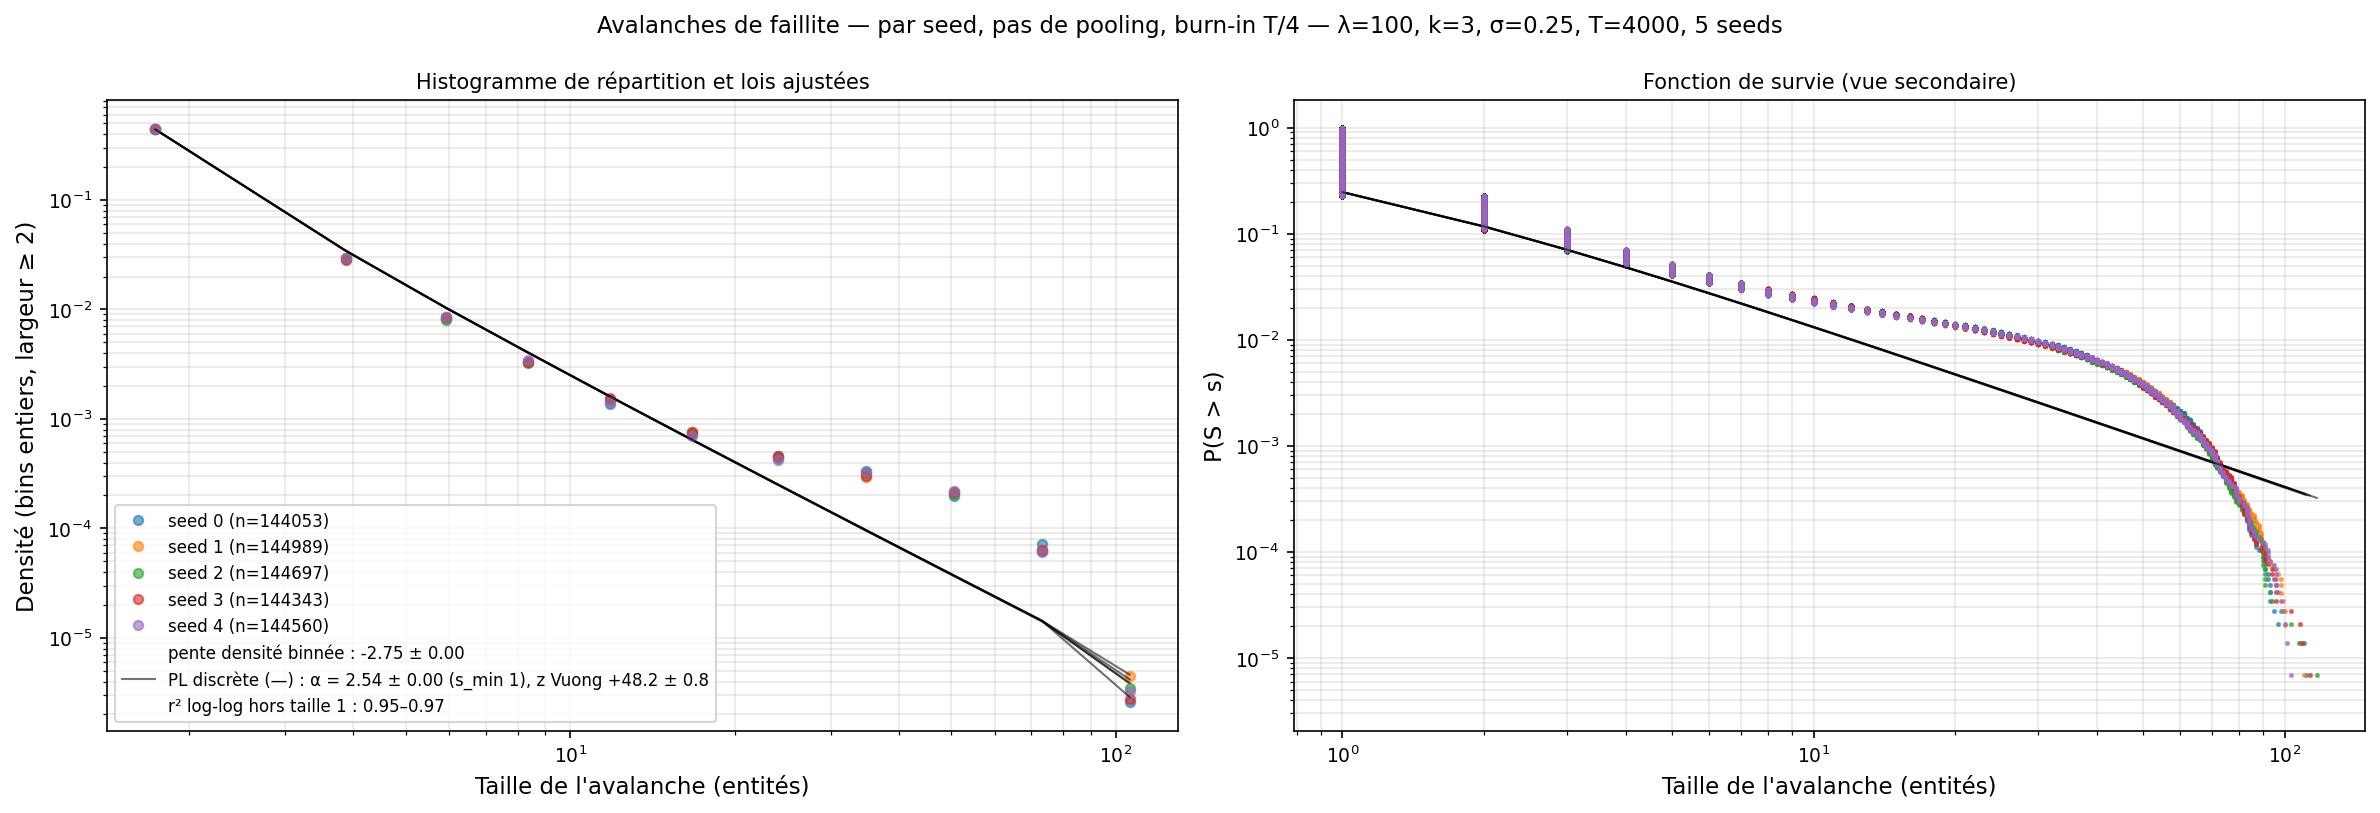
\includegraphics[width=0.98\textwidth]{figures/lot100_cascades_hist.png}
\caption{Distribution des tailles d'avalanches (nombre d'entités mortes),
lot $\lambda{=}100$, $T{=}4000$, 5 seeds. Gauche : histogramme de densité
sur bins entiers de largeur $\ge 2$ (vue principale), avec la loi de
puissance discrète ajustée par MLE superposée
($p(s) \propto s^{-\alpha}$, trait noir) ; exposant $\alpha$, $z$ de
Vuong contre la log-normale discrète et $r^2$ hors taille~1 en légende.
Droite : fonction de survie $P(S > s)$ (vue secondaire) avec le même
ajustement. Illustre les critères 1 et 3 (lot \code{20260715\_155159}).}
\label{fig:hist-fits}
\end{figure}

\begin{figure}[htbp]
\centering
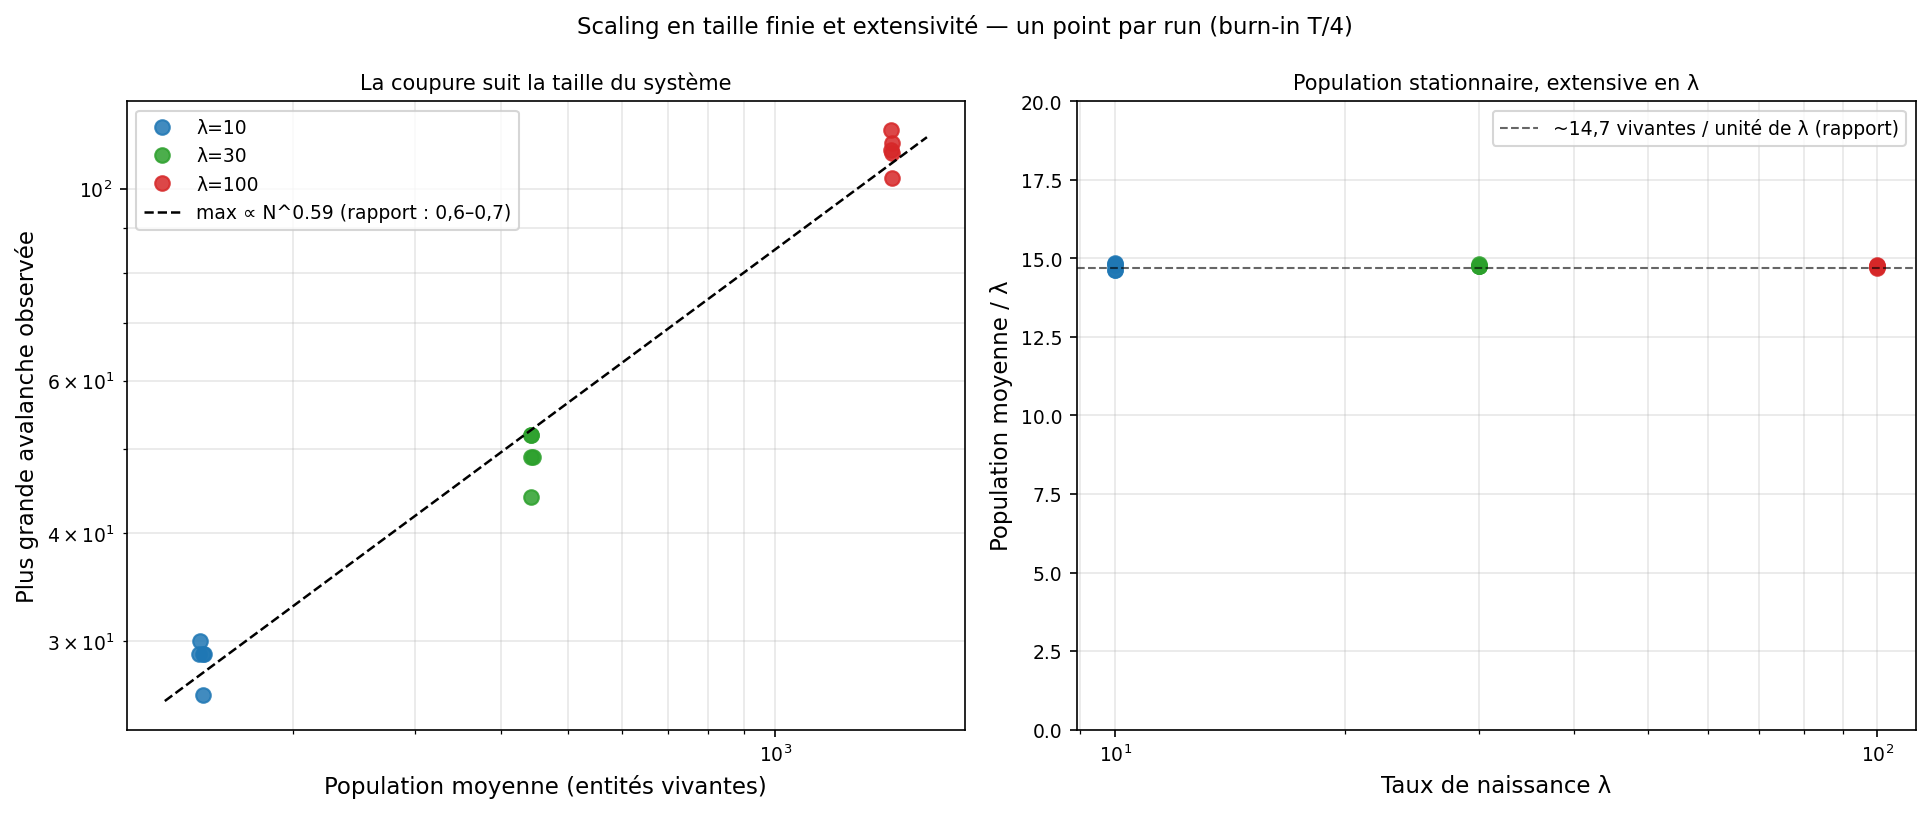
\includegraphics[width=0.95\textwidth]{figures/lots_scaling_finite_size.png}
\caption{Scaling en taille finie sur les trois lots ($T{=}4000$, 5 seeds
par lot) : à gauche, taille maximale d'avalanche par run en fonction de la
population moyenne $N$ (régression log-log : max $\propto N^{0{,}59}$,
critère 2 : la coupure suit la taille du système, sans saturation) ; à
droite, population stationnaire par unité de $\lambda$ (${\sim}14{,}7$,
extensivité). Calculé sur les trois lots de l'annexe~\ref{sec:annexe-lots}
(recettes de synthèse de \code{lab/batch\_report.py}).}
\label{fig:scaling-lots}
\end{figure}

\begin{figure}[htbp]
\centering
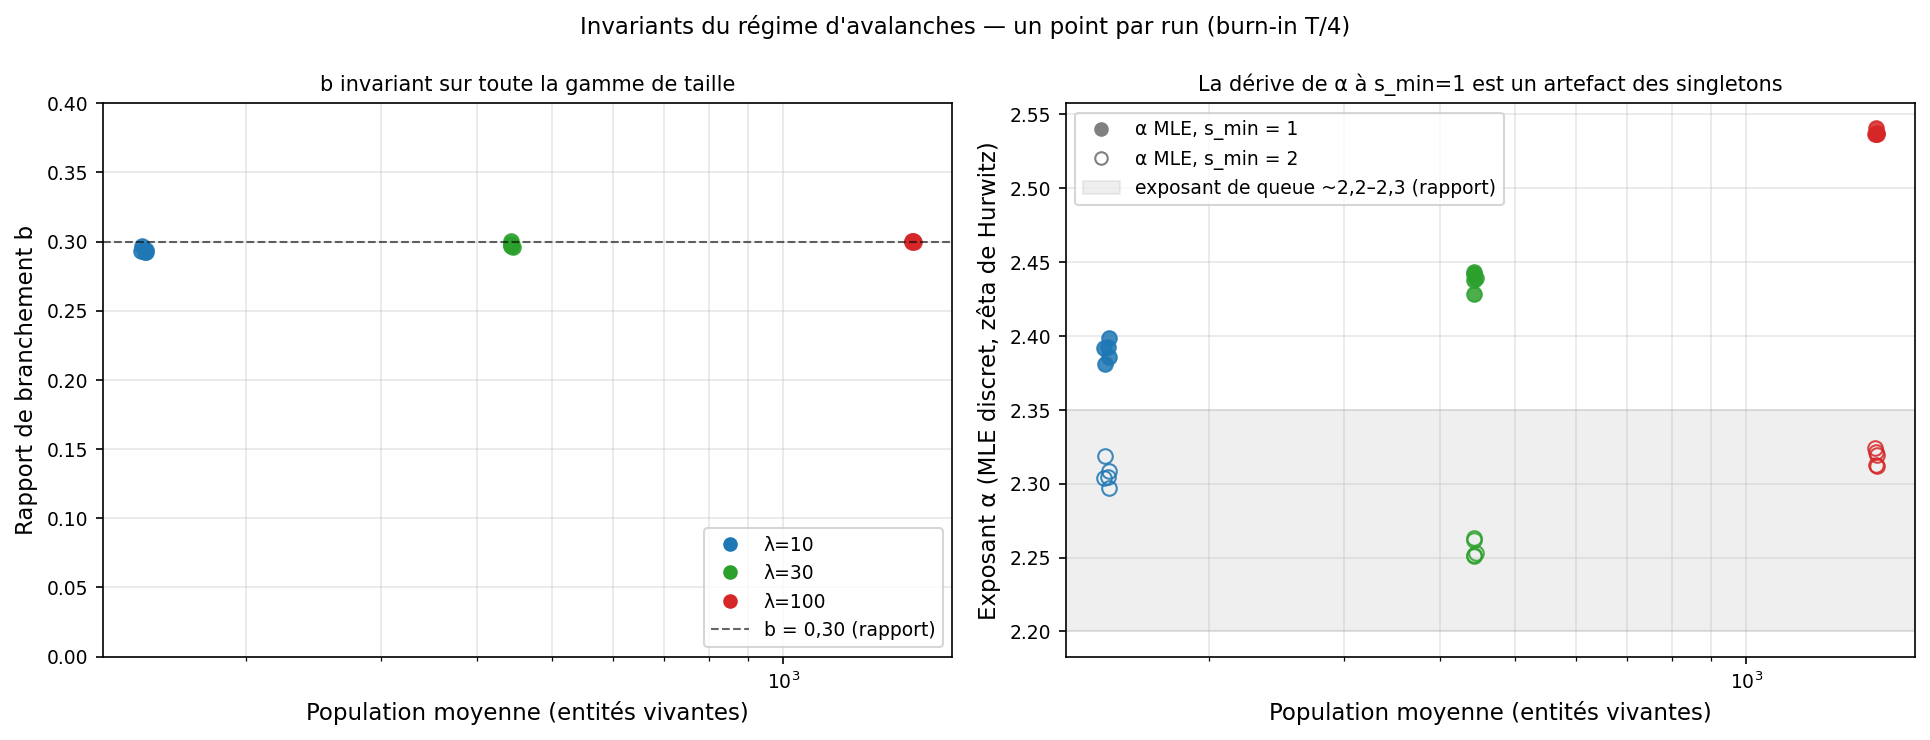
\includegraphics[width=0.95\textwidth]{figures/lots_invariants_soc.png}
\caption{Invariants à travers la gamme de tailles (un point par run) :
à gauche, rapport de branchement $b$ vs population moyenne --- $b$ reste
dans la bande $0{,}29$--$0{,}30$ sur toute la gamme ; à droite, exposant
$\alpha$ (MLE discret) au seuil $s_{\min}{=}1$ (symboles pleins, dérive
apparente $2{,}38 \to 2{,}54$ due au poids des singletons) et au seuil
$s_{\min}{=}2$ (symboles creux : $\alpha = 2{,}25$--$2{,}32$, stable ---
bande grisée $2{,}2$--$2{,}35$). Illustre le point « Exposant » ci-dessus.
Calculé sur les trois lots de l'annexe~\ref{sec:annexe-lots}.}
\label{fig:invariants}
\end{figure}

\begin{figure}[htbp]
\centering
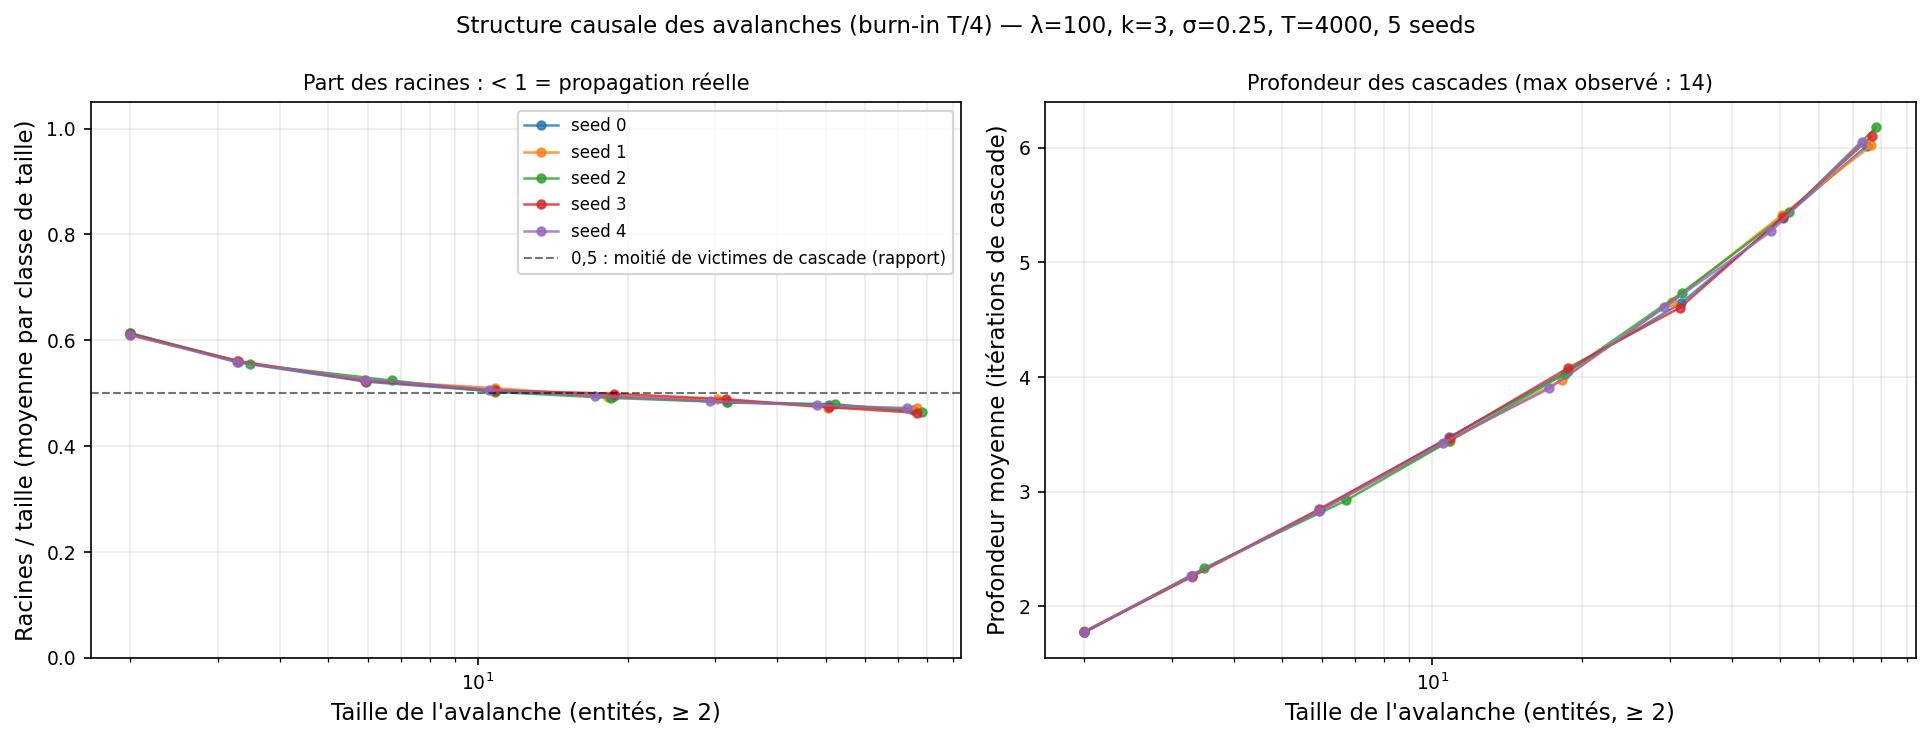
\includegraphics[width=0.95\textwidth]{figures/lot100_avalanche_structure.png}
\caption{Structure causale interne des avalanches, lot $\lambda{=}100$ :
rapport racines/taille (gauche) et profondeur de cascade (droite) en
fonction de la taille de l'avalanche. Les grands événements ont
racines/taille ${\sim}0{,}5$ (la moitié des membres sont des victimes
induites) et une profondeur qui croît jusqu'à 11--14 itérations : ce sont
des cascades de propagation, pas des grappes de morts synchronisées
(contraste avec le régime à chocs corrélés, §3.1). Lot
\code{20260715\_155159}.}
\label{fig:structure}
\end{figure}

\paragraph{Analyse causale inter-pas (exploratoire, à manier avec
précaution).} La mesure de référence (même pas) tronque la première
génération : une perte subie en phase 7 du pas $t$ n'est réévaluée qu'à la
résolution du pas $t+1$. Relier les morts par les arêtes de perte avec une
tolérance d'un pas ($\tau = 1$) est donc tentant, et sur le candidat
\emph{intermédiaire} (volume $n/3$, faible densité d'événements) cela révèle
des cascades multi-pas réelles : max 122 à pop.\ 517, 419 à pop.\ 1722,
$\alpha \approx 2{,}6$ sans coupure détectable. Mais cette mesure
\emph{percole} dès que la densité de liens est élevée : sur le contrôle à
règle M3, max 896 pour 233 vivantes (sur-liaison manifeste), et sur la
config \emph{finale} elle-même (moitié des morts en cascade), max 4006 à
$\lambda{=}30$ et $1{,}15 \cdot 10^5$ à $\lambda{=}100$ --- composante
géante, mesure inutilisable. Elle n'est donc PAS utilisée pour les
conclusions ; tous les chiffres de la table ci-dessus sont en mesure stricte
même-pas. Données : \code{loss\_edges.csv} par run ; analyse :
\code{causal\_window.py} (résultats \code{figures/causal\_window.json}).

\subsection{Le volume en joules des avalanches : loi de puissance au-dessus du mode}
\label{sec:volume}

Le \emph{volume} d'une avalanche est la somme des joules détruits par
l'événement (créances perdues $+$ actifs résiduels détruits des membres),
reconstruite depuis les arêtes de perte et les morts du pas. Au-dessus
d'un mode situé à ${\sim}110$--$120$~J, sa densité (bins logarithmiques)
suit une loi de puissance de pente $-2{,}12$ ($\lambda{=}10$) à
$-2{,}30$ ($\lambda{=}100$), très stable ($r^2 = 0{,}99$,
fig.~\ref{fig:vol-dp}). La partie montante de la densité (au-dessous du
mode), qui reflète la composition des petits événements plus que la
dynamique des avalanches, n'est pas analysée ici ; l'épaulement visible
avant la coupure à $\lambda{=}100$ n'est pas non plus interprété à ce
stade. Le fait notable est la position du mode :
\emph{indépendante de la taille du système} (régression du mode sur la
population : exposant $0{,}02$, fig.~\ref{fig:vol-exponents}) --- c'est
une échelle \emph{intensive}, de l'ordre de la valeur des expositions
individuelles autour de la cible de capital $K^*$, tandis que
l'extension de la queue suit la taille du système.

\begin{figure}[htbp]
\centering
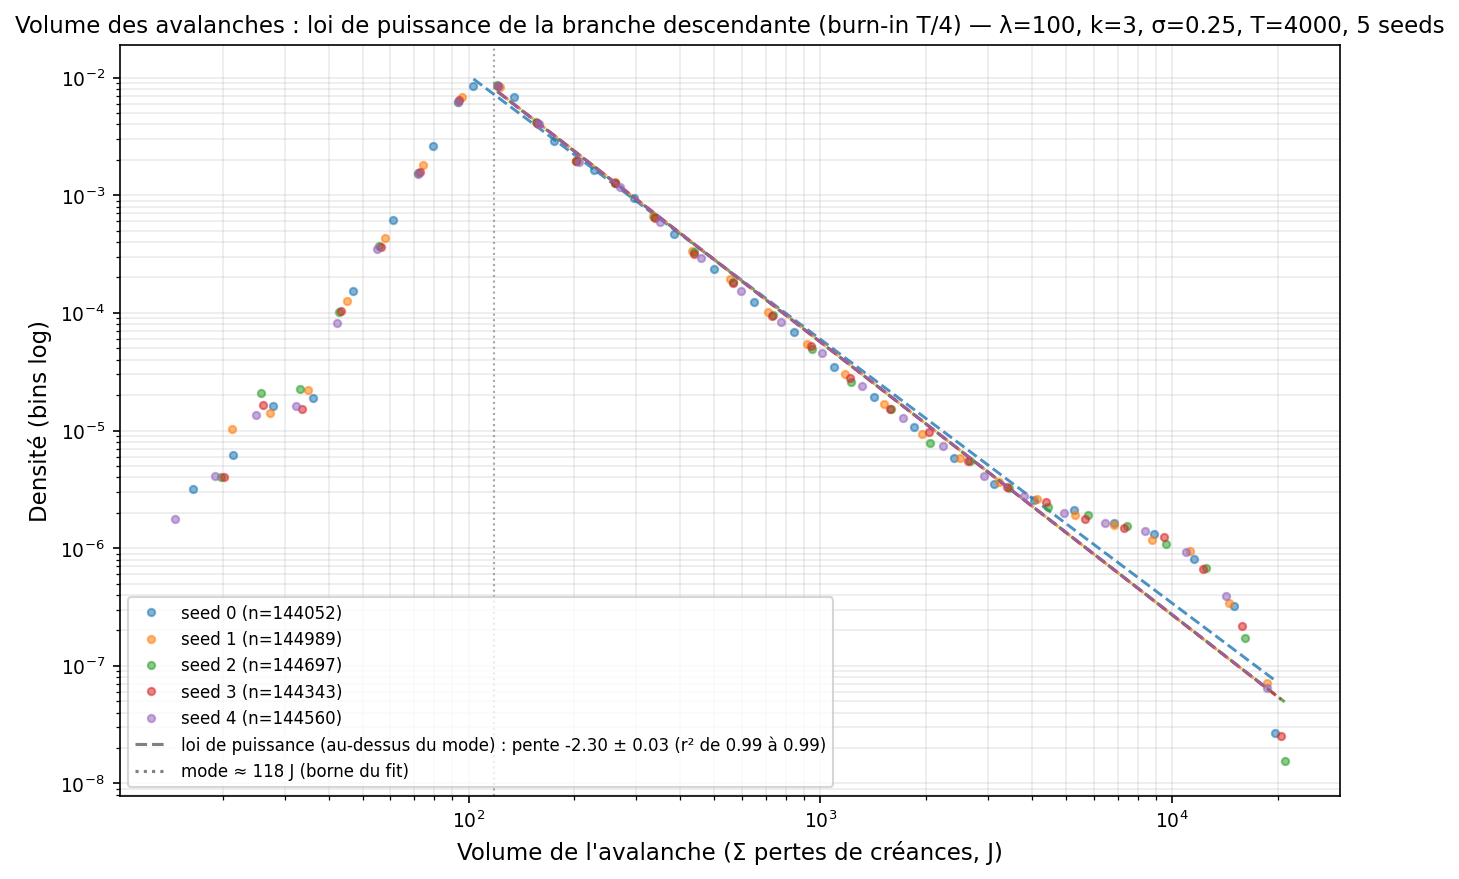
\includegraphics[width=0.98\textwidth]{figures/lot100_volume_double_pareto.png}
\caption{Densité du volume détruit par avalanche (J, bins
logarithmiques), lot $\lambda{=}100$, $T{=}4000$, 5 seeds. Régression
log-log de la branche descendante (au-dessus du mode, marqué en
pointillé) : pente et $r^2$ en légende. Lot \code{20260715\_155159}.}
\label{fig:vol-dp}
\end{figure}

\begin{figure}[htbp]
\centering
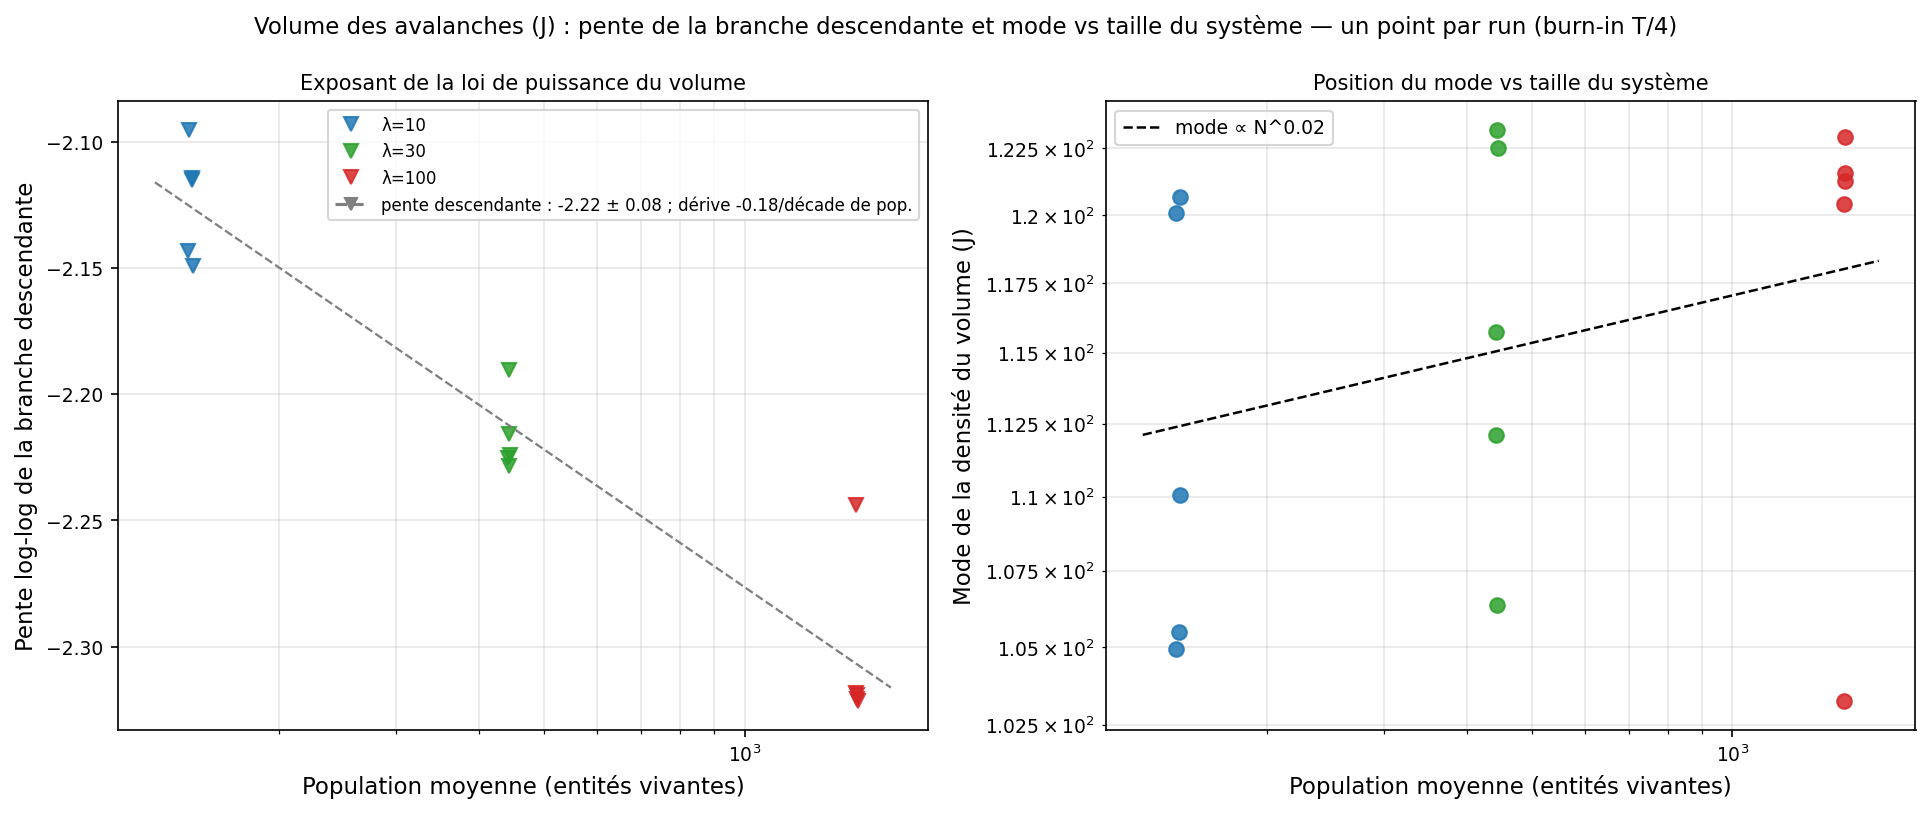
\includegraphics[width=0.95\textwidth]{figures/lots_volume_exponents.png}
\caption{Paramètres de la loi de puissance du volume vs taille du
système (un point par run, 3 lots $\times$ 5 seeds) : pente de la
branche descendante et position du mode vs population moyenne. La pente
est stable et le mode est indépendant de $N$ (exposant de régression
${\sim}0{,}02$) : le mode est fixé par l'échelle microscopique des
créances (${\sim}K^*$), pas par la taille du système. Calculé sur les
trois lots de l'annexe~\ref{sec:annexe-lots}.}
\label{fig:vol-exponents}
\end{figure}

\section{Ablations à un levier (contrôles)}

Autour du candidat intermédiaire (volume $n/3$, $\lambda = 30$, 3 seeds par
cellule ; mêmes conclusions qualitatives attendues autour de la config
finale) :

\begin{center}
\small
\begin{tabular}{lccccl}
\toprule
variante & max & rac./taille & prof.\ max & $r^2$ hors t.1 & verdict\\
\midrule
candidat (annul.\ $+$ destr.) & 23--30 & 0{,}44 & 7--8 & 0{,}97--0{,}99 & référence\\
destruction seule & 43--52 & 0{,}75 & 7--8 & 0{,}17--0{,}36 & \textbf{bosse} (pas une loi de puiss.)\\
annulation seule & 9--11 & 0{,}58--0{,}61 & 4--5 & 0{,}97--0{,}99 & propagation faible ($\alpha \approx 4{,}5$)\\
règle M3 (transf.\ $+$ prorata) & 27--31 & \textbf{0{,}93} & \textbf{3} & 0{,}92--0{,}94 & pas de propagation\\
objectif richesse ($\rho = r{+}\delta$) & 2 & --- & --- & --- & \textbf{pop.\ divergente}, aval.\ éteintes\\
naissance par emprunt & 25--27 & 0{,}44--0{,}45 & 7--9 & 0{,}98--1{,}00 & $\equiv$ candidat (option, défaut off)\\
$k = 2$ & 32--34 & 0{,}46--0{,}47 & 8--12 & 0{,}98--1{,}00 & fonctionne aussi ($\alpha \approx 2{,}65$)\\
$k = 6$ & 9--12 & 0{,}36--0{,}41 & 6--7 & 0{,}98--1{,}00 & propagation présente, queue courte\\
$\rho_s = 0{,}8$ ajouté & 93--117 & 0{,}47--0{,}48 & 9--10 & 0{,}99 & ajoute des déclencheurs, pas nécessaire\\
\bottomrule
\end{tabular}
\end{center}

Lectures : (i) c'est bien la \emph{combinaison} annulation $+$ destruction
qui porte le régime ; (ii) la règle de revenu est une condition d'existence
(l'objectif richesse fait diverger la population --- levier trop faible pour
que la dette tue) ; (iii) le régime n'exige pas de réglage fin de $k$
(2 et 3 fonctionnent, 6 raccourcit la queue via le tri assortatif plus
fort) ; (iv) la corrélation sectorielle n'est pas nécessaire et n'est pas le
mécanisme --- elle ne fait qu'ajouter des déclencheurs synchronisés.

\section{Contraintes du programme : préservées ; lois distributionnelles précisées}
\label{sec:distributions}

Sur la config finale ($\lambda = 30$ et $100$, dernier instantané,
\code{dist\_checks.py}) : corps de $\NW$ en Fisk (3 runs sur 4 ; 1 gamma),
corps de $K$ en Fisk (4/4), revenu en dPlN (3/4 ; 1 gamma) --- les familles
de M2/M3 et des lois réelles de référence ; Gini($\NW$) $= 0{,}42$--$0{,}44$
(fig.~\ref{fig:gini}) ;
renouvellement complet du top décile entre mi-parcours et fin (persistance
0,00 sur 1000 pas — l'espérance de vie est de ${\sim}15$ pas ;
fig.~\ref{fig:renewal}). La
population est stationnaire et extensive en $\lambda$ (${\sim}14{,}7$
vivantes par unité de $\lambda$, fig.~\ref{fig:scaling-lots}).

L'analyse approfondie sur les lots $T{=}4000$ (5 seeds par $\lambda$,
ajustements par seed --- jamais de mise en commun inter-seeds ---,
échantillons élargis aux 5 derniers instantanés espacés d'au moins 150
pas, soit dix fois l'espérance de vie : populations quasi indépendantes en
régime stationnaire) \emph{précise} ces verdicts de famille, obtenus sur
corps tronqué et un seul instantané :

\begin{itemize}[nosep]
\item \textbf{Revenu brut} (production $+$ intérêts nets, J/pas),
  ajusté sur les revenus $> 10$~J : \textbf{corps exponentiel $\times$
  queue Pareto, 5 seeds sur 5 sur chacun des trois lots}
  (fig.~\ref{fig:revenue}). Le modèle composite à 3 paramètres ---
  densité $\propto e^{-(x - 10)/T}$ jusqu'à un raccord $x_b$, puis
  $\propto x^{-\alpha}$ au-delà, continue en $x_b$ --- bat par AIC la
  log-normale ($\Delta$AIC $+70$ à $+800$ par seed), la gamma et
  l'exponentielle pure, sur les trois lots. Paramètres à
  $\lambda{=}100$ : $T = 22{,}3 \pm 1{,}6$~J/pas, $x_b = 25{,}1 \pm
  0{,}5$~J, $\alpha = 8{,}96 \pm 0{,}28$ ($r^2 = 0{,}96$--$0{,}97$) ;
  à $\lambda{=}30$ : $T = 24{,}8 \pm 6{,}7$, $x_b = 24{,}5 \pm 0{,}8$,
  $\alpha = 8{,}5 \pm 0{,}6$ ; à $\lambda{=}10$ : $x_b = 25{,}8 \pm
  2{,}4$, $\alpha = 10{,}4 \pm 2{,}6$ ($T$ mal contraint,
  $28 \pm 21$). Le raccord $x_b \approx 25$~J est stable à travers la
  gamme de tailles. La queue Pareto est raide ($\alpha \approx
  8{,}5$--$10$) : ce n'est pas une queue « sans échelle » au sens des
  avalanches, mais elle est mieux décrite par une loi de puissance que
  par la coupure log-normale testée précédemment.
\item \textbf{Capital productif $K$}, plein échantillon (sans troncature
  au corps ; familles à $\le 3$ paramètres libres, MLE) : \textbf{Burr
  XII, 5/5 sur les trois lots} (à $\lambda{=}100$ : paramètres de forme
  $c = 17{,}2 \pm 0{,}3$ et $d = 0{,}58 \pm 0{,}02$, échelle
  $104 \pm 1$~J ; $r^2$ pondéré $0{,}83$--$0{,}87$). Le pic étroit sur
  l'attracteur $K^*$ domine le fit ; le plateau des petits capitaux
  (entités jeunes ou déstabilisées, ${\sim}10\,\%$ de la masse) reste
  au-dessus de la courbe --- aucune famille simple ne capture les deux
  échelles à la fois (fig.~\ref{fig:distfits}).
\item \textbf{Valeur nette $\NW$}, plein échantillon : \textbf{gamma
  généralisée} (gengamma, 3 paramètres, dont la gamma est le cas
  particulier) --- gengamma 5/5 à $\lambda{=}100$ ($r^2 =
  0{,}97$--$0{,}98$), gengamma/gamma se partageant les seeds aux
  tailles inférieures (gamma 4/5 à $\lambda{=}10$) : la famille robuste
  est la gamma (généralisée), forme ${\sim}1{,}4$--$1{,}7$
  (fig.~\ref{fig:distfits}).
\item \textbf{Âge au décès} : \textbf{log-normal}, sur les deux
  échantillons --- toutes les morts ($\sigma_{\log} \approx 1{,}06$,
  médiane ${\sim}8{,}3$ pas) et les morts d'âge $> 5$ recalées de $-5$
  ($\sigma_{\log} \approx 1{,}14$, médiane ${\sim}10{,}4$ pas), $r^2 =
  0{,}97$--$0{,}99$ sur les 5 seeds (fig.~\ref{fig:age}). La densité est
  convexe en semi-log sur deux décades : aucune exponentielle ne peut la
  suivre --- \textbf{la mortalité n'est pas sans mémoire}, le risque de
  décès dépend de l'âge, cohérent avec l'accumulation progressive de
  levier.
\end{itemize}

\begin{figure}[htbp]
\centering
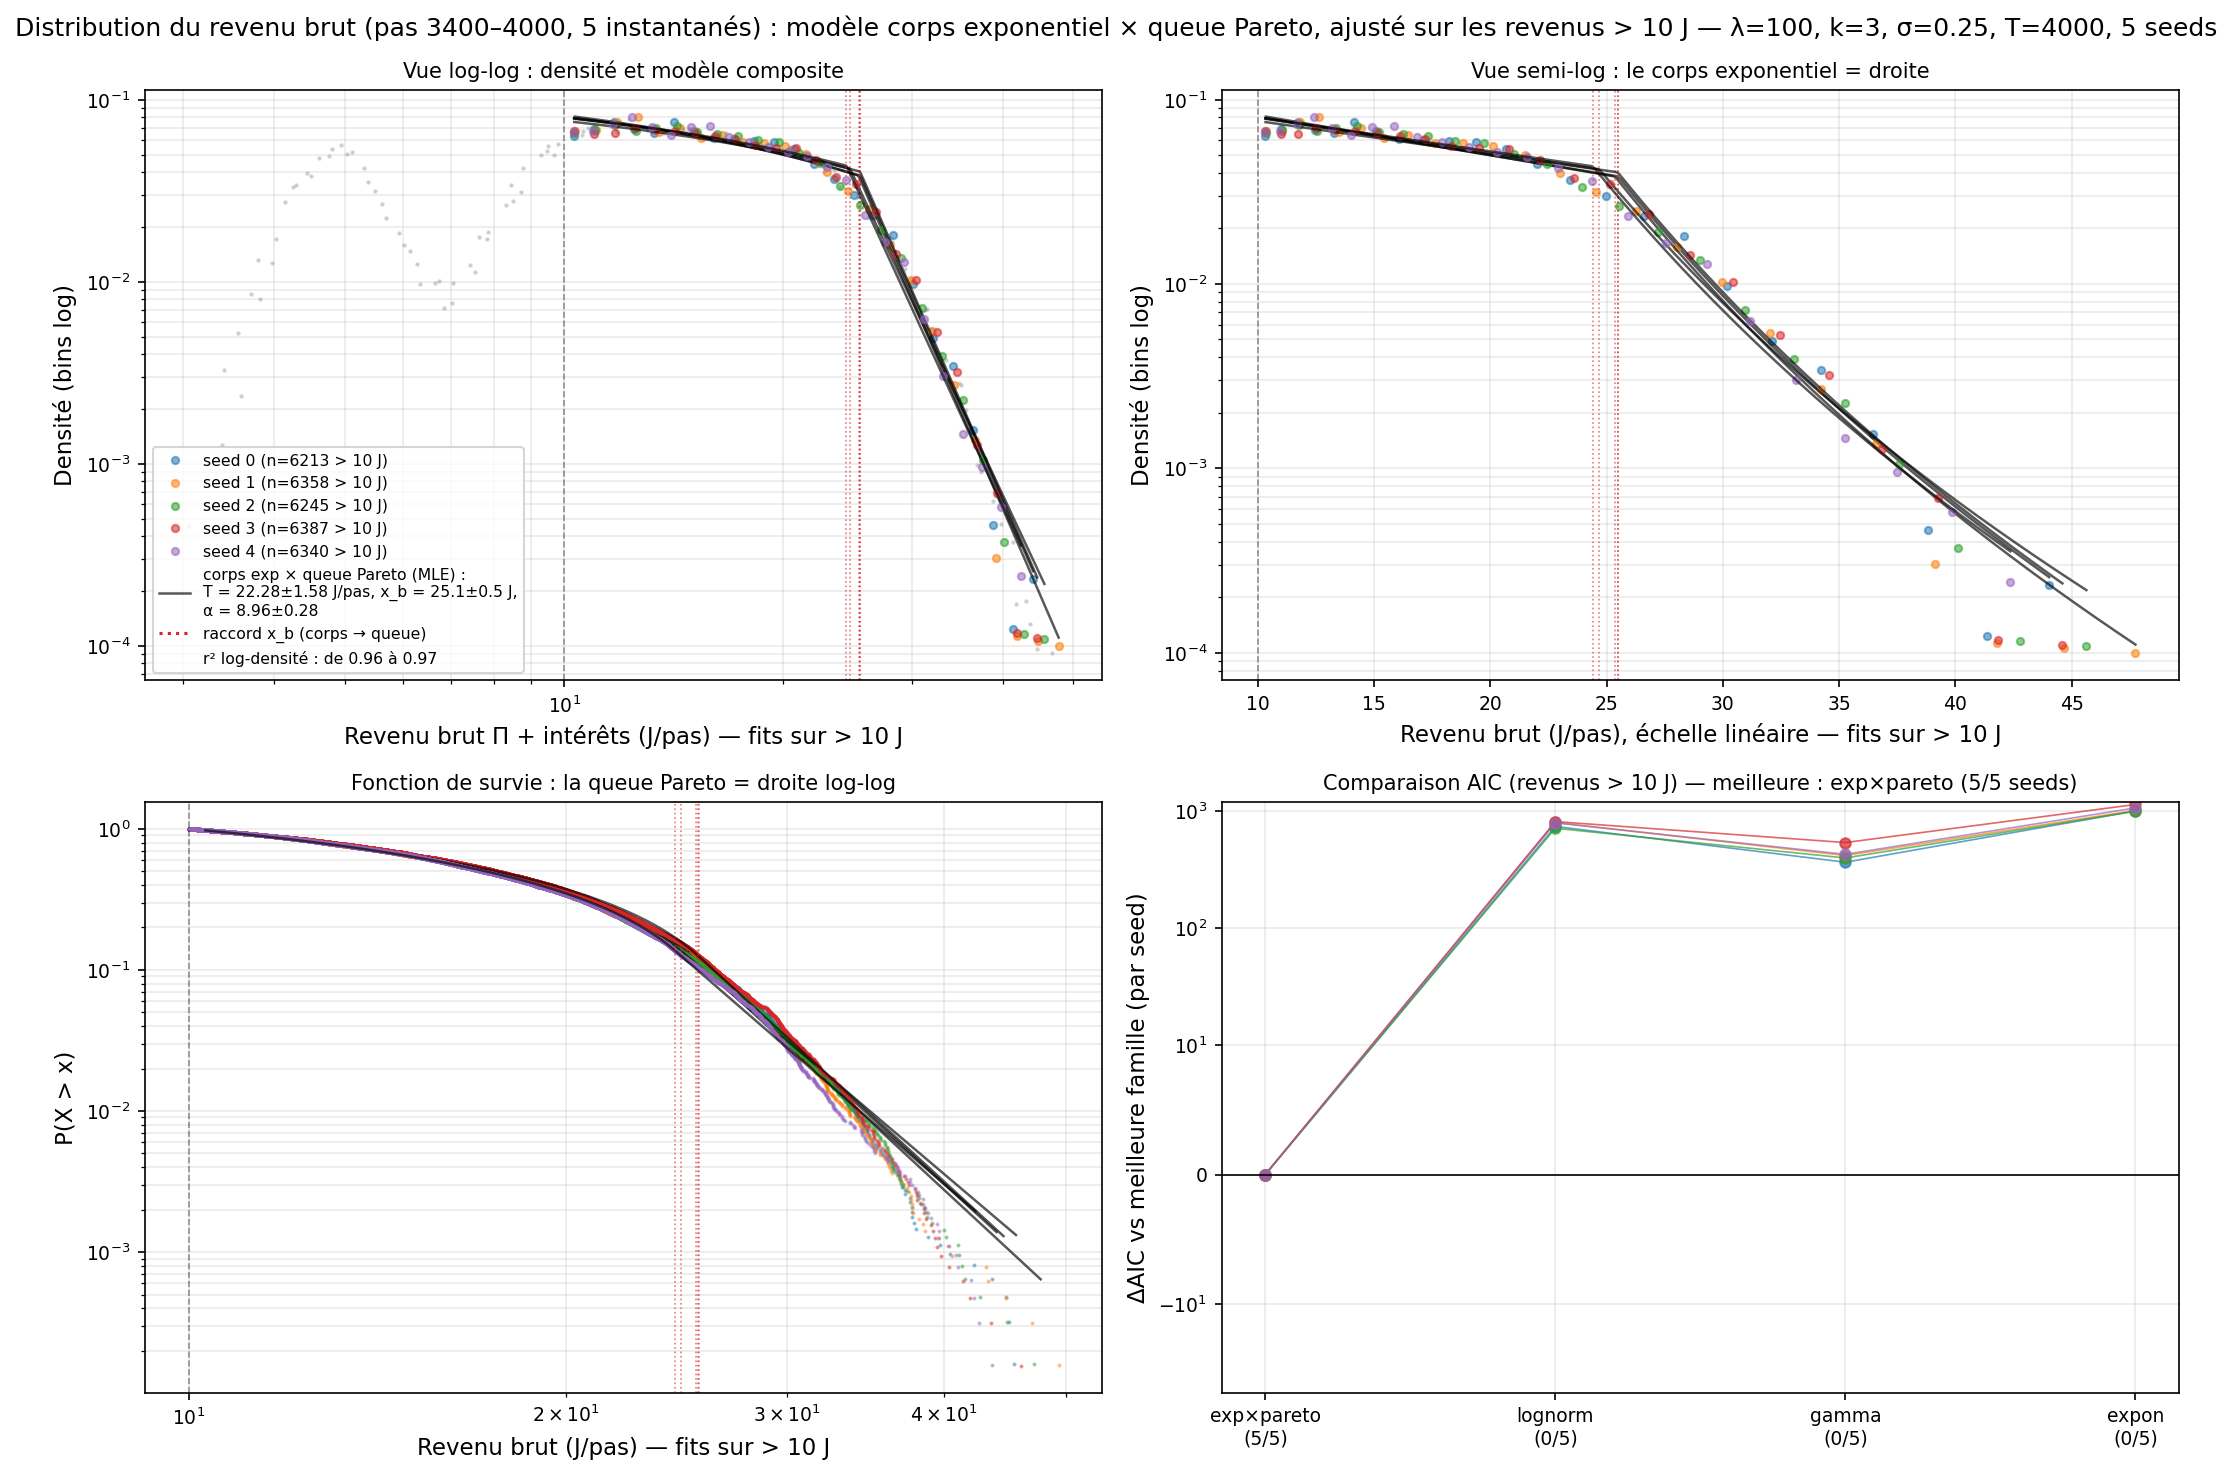
\includegraphics[width=0.98\textwidth]{figures/lot100_revenue_fits.png}
\caption{Distribution du revenu brut (J/pas), lot $\lambda{=}100$,
$T{=}4000$, 5 seeds, modèle « corps exponentiel $\times$ queue Pareto »
ajusté par MLE par seed sur les revenus $> 10$~J (densité complète en
gris ; raccord $x_b$ en pointillé rouge). Haut gauche : vue log-log,
paramètres et $r^2$ en légende. Haut droite : vue semi-log --- le corps
exponentiel y est une droite. Bas gauche : fonction de survie log-log
--- la queue Pareto y est une droite. Bas droite : comparaison AIC ---
le modèle composite gagne 5/5 contre log-normale, gamma et exponentielle
pure. Lot \code{20260715\_155159}.}
\label{fig:revenue}
\end{figure}

\begin{figure}[htbp]
\centering
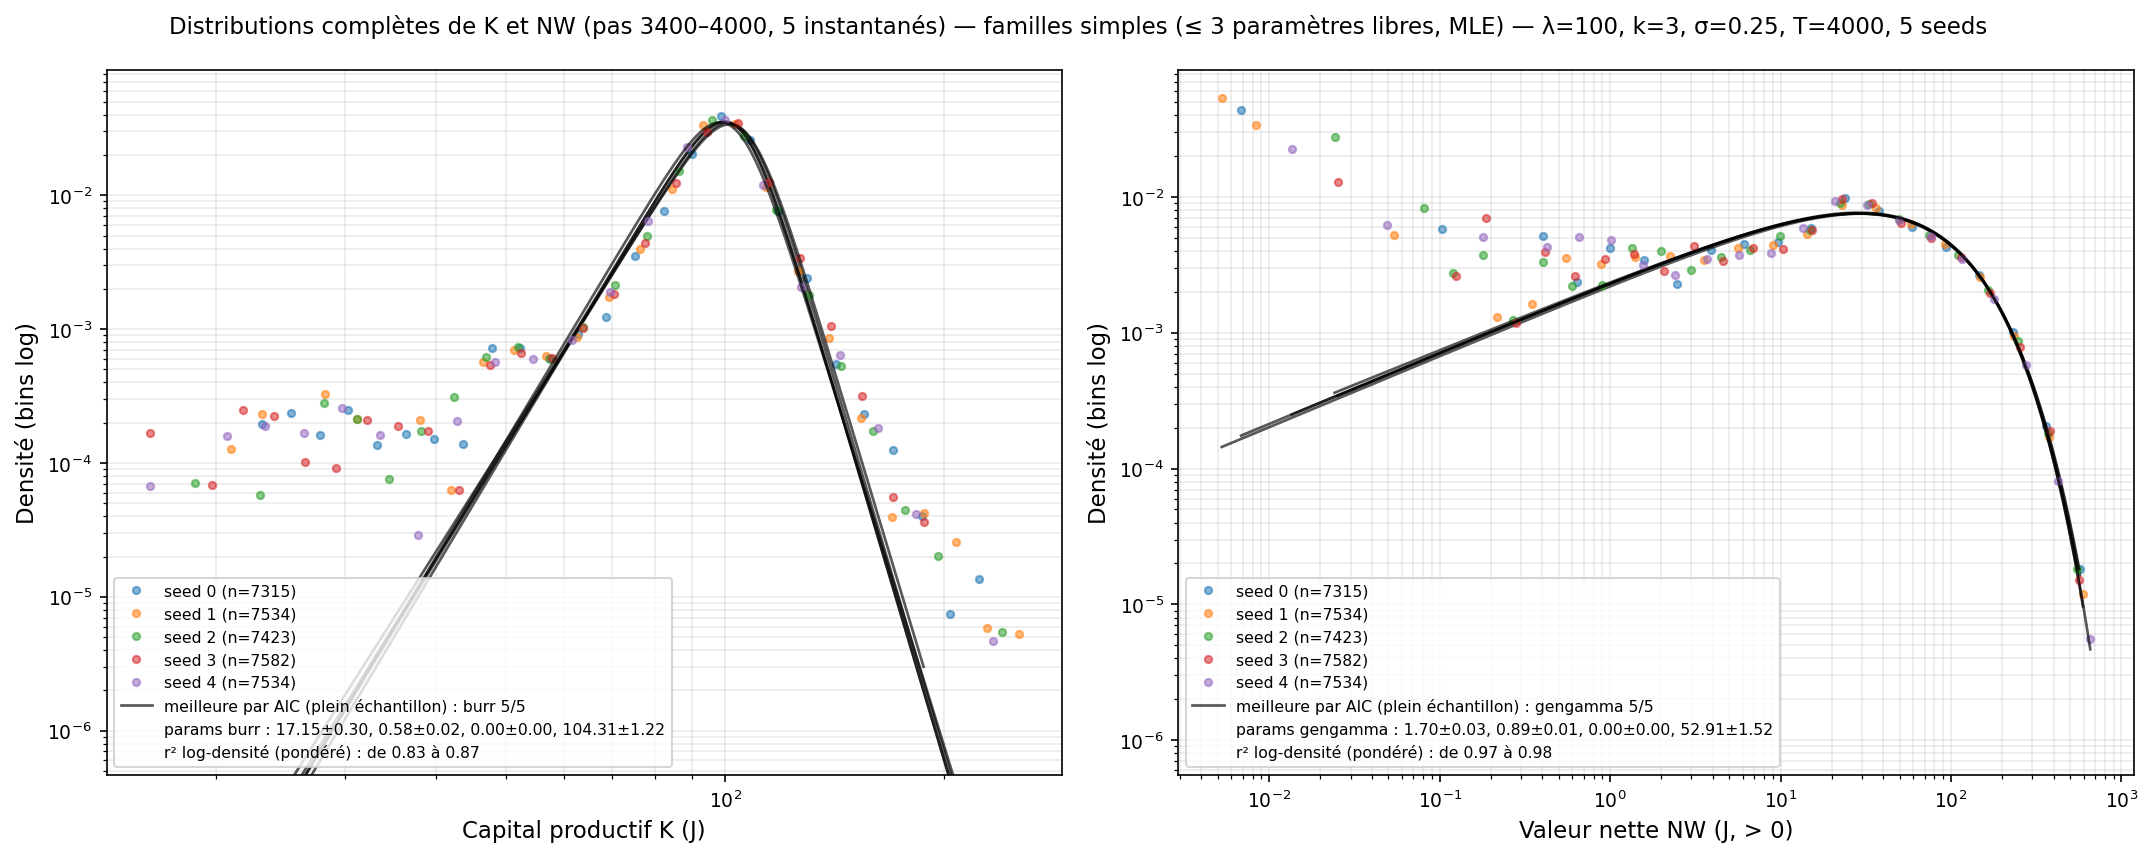
\includegraphics[width=0.98\textwidth]{figures/lot100_distribution_fits.png}
\caption{Distributions de taille des entités, plein échantillon (5
instantanés tardifs par seed), lot $\lambda{=}100$ : capital productif
$K$ (gauche) et valeur nette $\NW$ (droite), meilleure famille par AIC
parmi les lois simples à $\le 3$ paramètres libres (MLE, paramètres et
$r^2$ pondéré en légende). $K$ : Burr XII 5/5 (le plateau des petits
capitaux reste au-dessus du fit) ; $\NW$ : gamma généralisée 5/5. Lot
\code{20260715\_155159}.}
\label{fig:distfits}
\end{figure}

\begin{figure}[htbp]
\centering
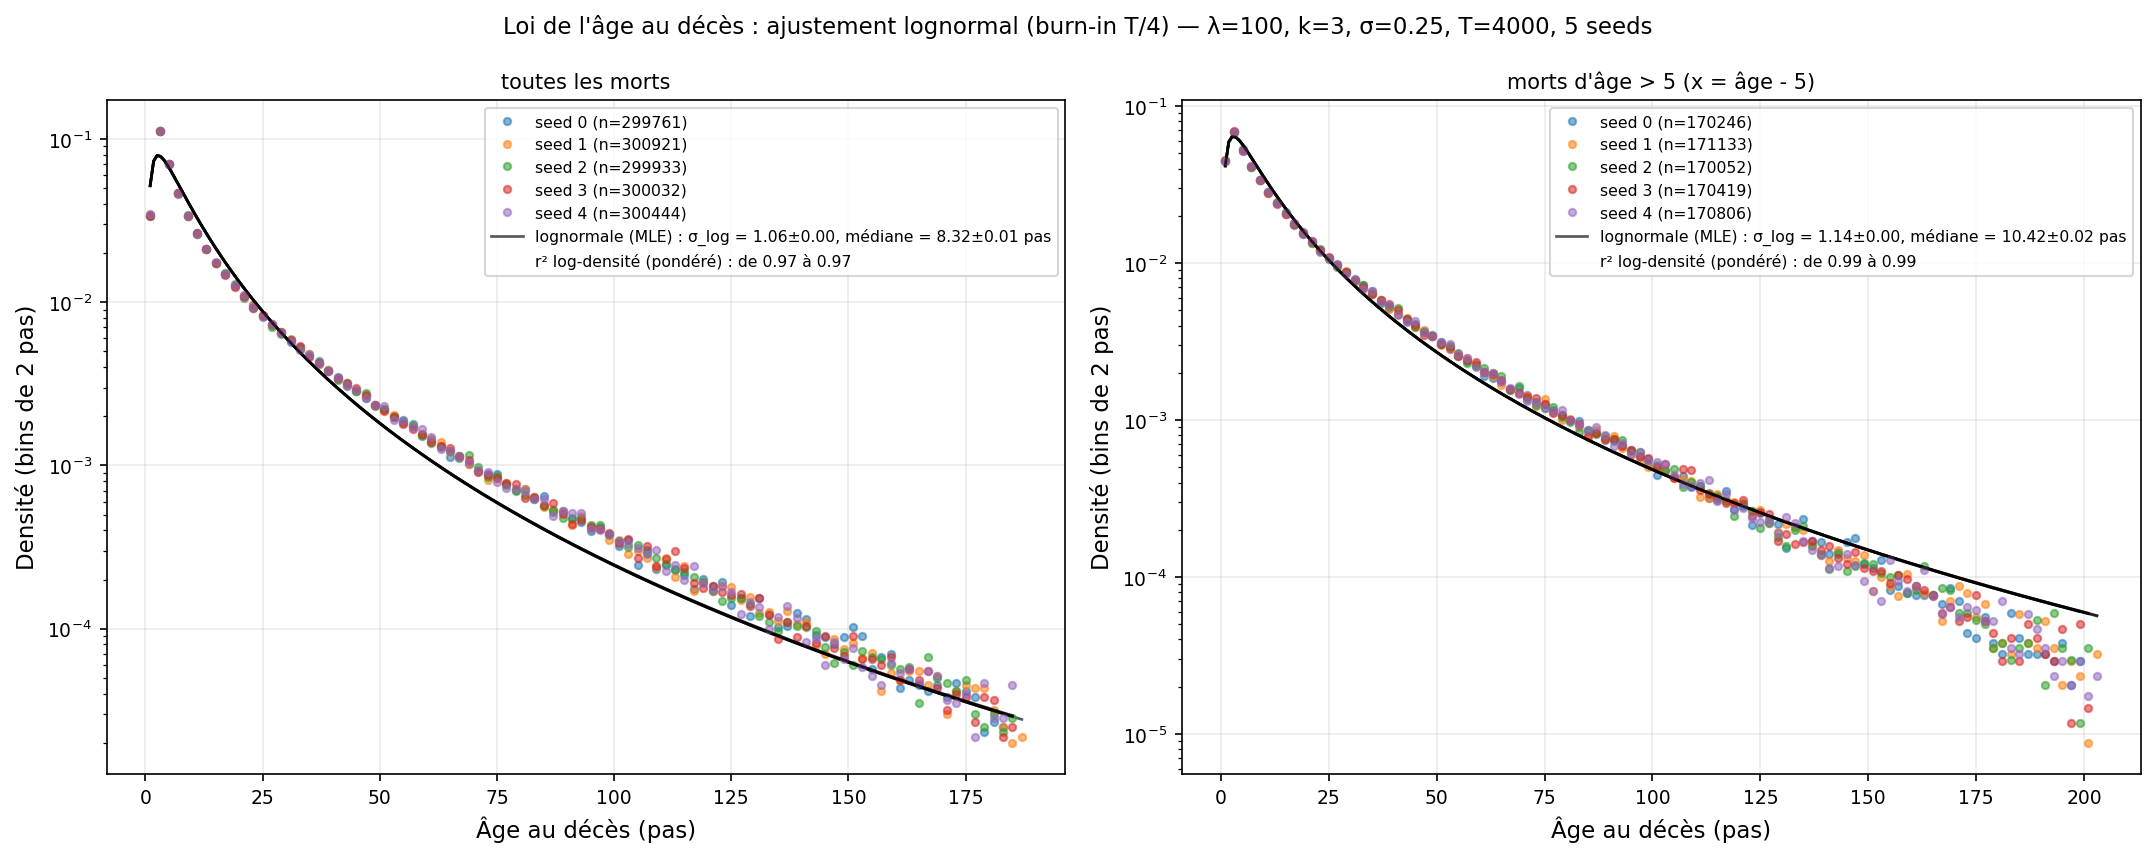
\includegraphics[width=0.98\textwidth]{figures/lot100_age_at_death_fits.png}
\caption{Loi de l'âge au décès, lot $\lambda{=}100$ (${\sim}3 \cdot 10^5$
morts par seed après burn-in) : toutes les morts (gauche) et morts d'âge
$> 5$ recalées ($x = \text{âge} - 5$, droite), densité sur bins de 2 pas
en échelle semi-log, ajustement log-normal par seed (trait noir ;
paramètres et $r^2$ pondéré en légende). La convexité de la densité en
semi-log exclut toute loi exponentielle (qui y serait une droite). Lot
\code{20260715\_155159}.}
\label{fig:age}
\end{figure}

\begin{figure}[htbp]
\centering
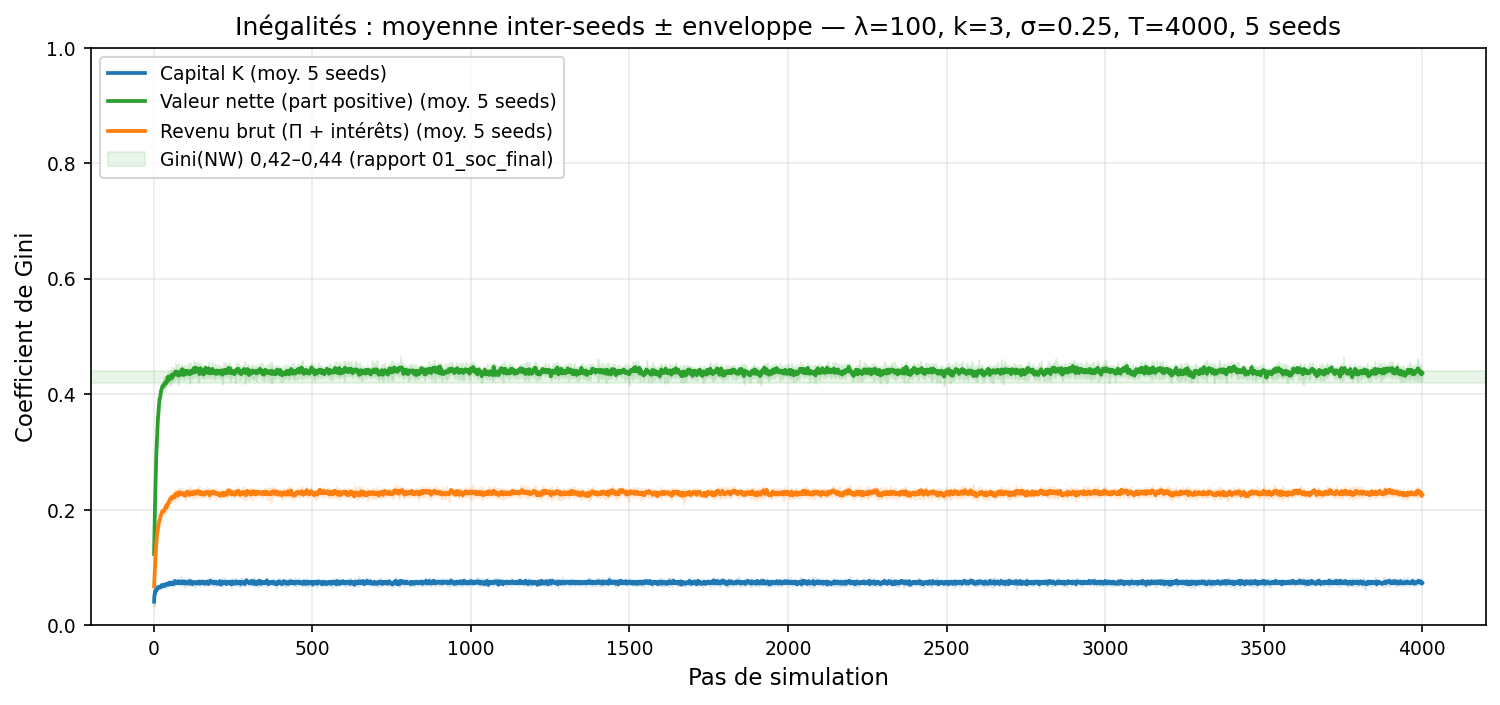
\includegraphics[width=0.9\textwidth]{figures/lot100_gini_evolution.png}
\caption{Indice de Gini de la valeur nette au cours du temps, lot
$\lambda{=}100$, 5 seeds ; la bande grisée marque la plage
$0{,}42$--$0{,}44$ annoncée ci-dessus : le Gini est stationnaire dans
cette bande après le burn-in. Lot \code{20260715\_155159}.}
\label{fig:gini}
\end{figure}

\begin{figure}[htbp]
\centering
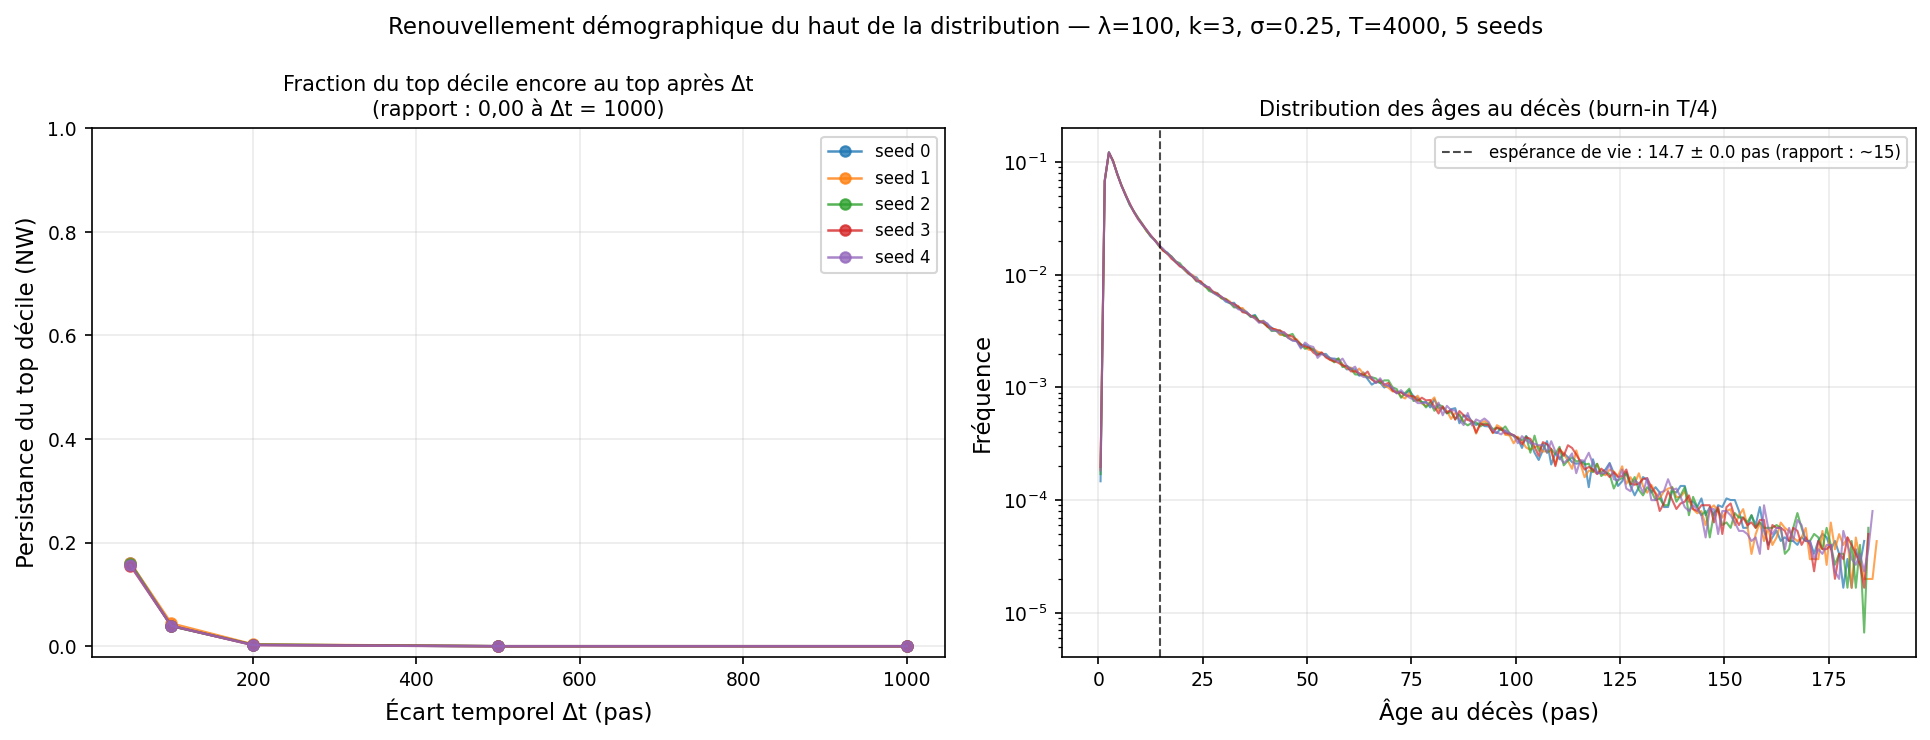
\includegraphics[width=0.95\textwidth]{figures/lot100_top_decile_renewal.png}
\caption{Renouvellement du haut de la distribution, lot $\lambda{=}100$ :
persistance du top décile (fraction des entités du top décile de $\NW$ à
$t$ encore dans le top décile à $t + \Delta t$) pour $\Delta t \in \{50,
100, 200, 500, 1000\}$ --- inférieure à $0{,}2$ dès $\Delta t = 50$ et
nulle au-delà de $\Delta t = 200$ ---, et histogramme de l'âge au décès.
Le haut de la distribution se renouvelle entièrement ; il n'y a pas
d'oligarchie persistante. Lot \code{20260715\_155159}.}
\label{fig:renewal}
\end{figure}

\section{Limites, et statut de la revendication « SOC »}

\begin{itemize}[nosep]
\item \textbf{Ce qui est auto-organisé} : à institution de marché donnée,
  le rapport de branchement $b$ est un invariant dynamique
  ($0{,}287$--$0{,}301$ sur 30$\times$ la gamme de taille --- et
  $0{,}300 \pm 0{,}001$ dès $\lambda \ge 30$ --- tous seeds, insensible à
  $\sigma$), la coupure suit la taille du système, et l'exposant est
  reproductible. Aucun paramètre n'est ajusté \emph{vers} la criticité
  pendant le run.
\item \textbf{Ce qui reste institutionnel} : la position de la fenêtre
  critique dépend du volume d'appariement (un round par tête). C'est un
  choix de structure comparable à la connectivité d'un réseau dans un
  modèle de tas de sable --- large d'un facteur ${\sim}2$, pas un réglage
  fin --- mais un marché « sur-apuré » ($\ge 2$ rounds/tête) dépasse le
  point critique. La revendication honnête est donc : \emph{criticité
  auto-entretenue dans une fenêtre institutionnelle large}, pas attracteur
  universel indépendant de l'institution.
\item $b = 0{,}30 \ne 1$ : les avalanches ne sont pas un processus de
  branchement critique au sens strict ; la loi de puissance émerge de la
  combinaison propagation ($b$) $\times$ fan-in des créancières communes
  $\times$ hétérogénéité des expositions. La théorie du « pourquoi
  $\alpha \approx 2{,}5$ » reste ouverte.
\item L'exposant $\alpha$ dérive de 2,40 à 2,63 avec la taille du système ;
  correction de taille finie probable mais non démontrée.
\item La famille du revenu, incertaine dans la version initiale (dPlN
  3/4, gamma 1/4), est tranchée par les lots $T{=}4000$ : corps
  exponentiel $\times$ queue Pareto au-dessus de 10~J, 5/5 sur les trois
  lots (§\ref{sec:distributions}). La queue Pareto est raide
  ($\alpha \approx 8{,}5$--$10$) : les vies courtes (${\sim}15$ pas) ne
  laissent pas le temps au mécanisme multiplicatif de construire une
  queue lourde --- un écart assumé aux familles observées dans M3 (vies
  longues).
\end{itemize}

\section{Traçabilité}

Moteur : \code{src/m4/} (fusionné, $d_0$ retiré) ; état pré-refonte archivé
dans \code{archive/m4\_lk\_pre\_refonte/}. Tests : \code{tests/} (61).
Journal : \code{NOTES.md} (une entrée par hypothèse, y compris les
négatifs). Figures de synthèse :
\code{experiments/m4/report\_figures/} (+ \code{sources.json}).

{\small
\begin{longtable}{lll}
\toprule
run\_id & rôle & config clé (sinon défauts finaux)\\
\midrule
\code{m4\_first\_s0} & point de départ (max 7) & moteur L/K, $\rho_s{=}0{,}8$, $d_0{=}28$, $\lambda{=}10$\\
\code{a1\_lam\{10,30,100\}p0\_s\{0-2\}} & baseline fork M3, scaling & moteur L/K, $\rho_s{=}0{,}8$\\
\code{a2\_shock\_rho\_sector*\_s\{0-2\}} & dose-réponse $\rho_s$ (amplification) & moteur L/K, $\lambda{=}30$\\
\code{a3\_n\_sectors\{2,10,20\}\_s\{0-2\}} & cutoff vs taille de secteur & moteur L/K, $\lambda{=}30$\\
\code{b\_lam\{10,30\}p0\_s\{0-2\}} & plancher endogène $d_0{=}0$ & moteur L/K, $\lambda{=}10/30$\\
\code{c\_lam\{10,30,100\}\_s\{0-2\}} & candidat intermédiaire (rounds $n/3$) & fusionné, \code{rounds\_div=3}\\
\code{ct\_lam30\_T4000\_s\{0-2\}} & robustesse $T$ & fusionné, \code{rounds\_div=3}\\
\code{v\_r\{6,3,2\}\_s\{0-2\}} & dose-réponse volume $\to b$, $x_c$ & fusionné, $\lambda{=}30$\\
\code{f\_lam\{10,30,100\}\_s\{0-2\}} & \textbf{campagne confirmatoire finale} & défauts finaux, $T{=}2000$\\
\code{f\_lam30\_T4000\_s\{0-2\}} & robustesse $T$ (finale) & défauts finaux\\
\code{f\_lam300\_s0} & scaling extrême & défauts finaux, $\lambda{=}300$\\
\code{abl\_cancel\_only\_s\{0-2\}} & ablation : annulation seule & \code{fail\_residual=prorata}$^\dagger$\\
\code{abl\_destroy\_only\_s\{0-2\}} & ablation : destruction seule & \code{fail\_lender\_loans=transfer}$^\dagger$\\
\code{abl\_m3rule\_s\{0-2\}} & contrôle : règle M3 complète & transfer $+$ prorata$^\dagger$\\
\code{abl\_wealth\_s\{0-2\}} & contrôle bas levier (divergente) & \code{objective=wealth}$^\dagger$\\
\code{abl\_birthloan\_s\{0-2\}} & naissance par emprunt & \code{birth\_loan=True}$^\dagger$\\
\code{abl\_k\{2,6\}\_s\{0-2\}}, \code{abl\_sector\_s\{0-2\}} & robustesse $k$, contrôle $\rho_s$ & variantes$^\dagger$\\
\bottomrule
\end{longtable}
}

$^\dagger$~Les cellules d'ablation (\code{abl\_*}) ont été lancées avec le
volume \emph{intermédiaire} (\code{rounds\_div=0} $\to$ $n/k$ rounds), pas
avec le volume final ($n$ rounds) --- leurs verdicts qualitatifs (nécessité
des deux règles de faillite, de la règle de revenu, non-nécessité de la
corrélation) portent sur le mécanisme, pas sur la position exacte de la
fenêtre critique. \code{abl\_wealth} s'arrête sur le garde-fou
\code{pop\_max} (statut « explosion », population divergente).

Tous les runs : \code{experiments/m4/results/<run\_id>/}
(\code{config.json}, \code{series.csv}, \code{avalanches.csv},
\code{loss\_edges.csv} pour les runs f/v/abl, instantanés \code{.npz},
\code{figures/soc\_stats.json}). Les scans prototypes (jetables,
\code{proto\_*.log}) ont servi à l'exploration ; \textbf{toute conclusion de
cette note s'appuie sur les runs moteur listés ci-dessus}, à l'exception de
la ligne $4n$ rounds de la dose-réponse (prototype seulement, marquée
« bosse »).

\subsection*{Annexe : lots Simulation Lab de la seconde campagne}
\label{sec:annexe-lots}

Les figures ajoutées le 17 juillet proviennent de trois lots exécutés via
l'interface Simulation Lab (modèle \code{m4\_credit\_soc\_fable},
configuration finale par défaut, seeds 0--4, $T = 4000$, burn-in $T/4$
pour toutes les statistiques) et de leur synthèse inter-lots. Artefacts :
\code{simulation\_lab\_data/runs/<lot>\_lot/} (figures $+$
\code{aggregate.json}) ; statistiques par run dans
\code{simulation\_lab\_data/runs/m4\_soc\_synthese\_lots/soc\_summary.json}.
Les figures de synthèse de cette note
(\ref{fig:scaling-lots}, \ref{fig:invariants}, \ref{fig:vol-exponents})
sont calculées sur les trois lots ci-dessous \emph{exclusivement} ; la
synthèse affichée dans l'interface peut inclure des lots exploratoires
supplémentaires. Régénération :
\code{m4\_credit\_soc\_fable/lab/batch\_report.py <batch\_id> --force}.

{\small
\begin{tabular}{llll}
\toprule
lot (\code{batch\_id}) & $\lambda$ & seeds & figures de cette note\\
\midrule
\code{20260715\_154537\_6c5c0014} & 10 & 0--4 &
  \ref{fig:scaling-lots}, \ref{fig:invariants}, \ref{fig:vol-exponents}\\
\code{20260715\_154731\_027e9fbb} & 30 & 0--4 &
  \ref{fig:accum} ; $+$ id.\ synthèse\\
\code{20260715\_155159\_76b0c26e} & 100 & 0--4 &
  \ref{fig:branching}, \ref{fig:hist-fits}, \ref{fig:structure},
  \ref{fig:vol-dp}, \ref{fig:revenue}, \ref{fig:distfits},
  \ref{fig:age}, \ref{fig:gini}, \ref{fig:renewal}\\
\code{m4\_soc\_synthese\_lots} & 10/30/100 & --- &
  \ref{fig:scaling-lots}, \ref{fig:invariants}, \ref{fig:vol-exponents}\\
\bottomrule
\end{tabular}
}

Les runs individuels des lots sont stationnaires (population bornée,
statut \code{completed}) ; toutes les lois ajustées le sont par seed, et
les légendes donnent moyenne $\pm$ écart-type inter-seeds des paramètres.

\end{document}
